\documentclass[10pt,a4paper]{article}
\usepackage[a4paper,margin=18mm,headheight=15pt,footskip=14mm]{geometry}
\usepackage{fontspec}
\setmainfont{Noto Sans}
\setsansfont{Inter}
\setmonofont{DejaVu Sans Mono}[Scale=0.88]
\usepackage{amsmath,amssymb,mathtools}
\usepackage{microtype}
\usepackage{xcolor}
\usepackage{graphicx}
\graphicspath{{figures/}}
\usepackage{booktabs,longtable,tabularx,array,multirow,colortbl}
\usepackage{enumitem}
\usepackage{fancyhdr}
\usepackage{titlesec}
\usepackage{caption}
\usepackage{float}
\usepackage{tcolorbox}
\tcbuselibrary{breakable,skins}
\usepackage{fvextra}
\usepackage{seqsplit}
\usepackage{hyperref}
\usepackage{bookmark}
\usepackage{lastpage}
\usepackage{tikz}
\usepackage{ragged2e}

\definecolor{UGTSNavy}{HTML}{0D2B3A}
\definecolor{UGTSTeal}{HTML}{16979B}
\definecolor{UGTSGold}{HTML}{D4A21B}
\definecolor{UGTSCoral}{HTML}{CF6A5A}
\definecolor{UGTSPurple}{HTML}{6B5D96}
\definecolor{UGTSGreen}{HTML}{3F8D6A}
\definecolor{UGTSLight}{HTML}{EDF6F6}
\definecolor{UGTSLightGold}{HTML}{FBF5E4}
\definecolor{UGTSLightPurple}{HTML}{F2EFF8}
\definecolor{UGTSGrey}{HTML}{66737B}
\definecolor{UGTSDark}{HTML}{15252E}

\hypersetup{
  colorlinks=true,
  linkcolor=UGTSTeal,
  urlcolor=UGTSPurple,
  citecolor=UGTSTeal,
  pdftitle={UGTS-KC 3.6 - Literal Referential Geometric-Topological Substrate},
  pdfauthor={Tom Klootwijk (requester-supplied attribution); technical synthesis generated by OpenAI},
  pdfsubject={Geometric definitions, topology, hinge calculus, Dutch phonetic-number profiles, literal substrate schema and reference implementation},
  pdfkeywords={UGTS, geometry, topology, kinematic calculus, hinge, Dutch numbers, phonetics, SDF, event calculus, referential schema}
}

\pagestyle{fancy}
\fancyhf{}
\fancyhead[L]{\sffamily\small\color{UGTSNavy}\textbf{UGTS-KC 3.6}}
\fancyhead[R]{\sffamily\small\color{UGTSGrey}Literal referential substrate}
\fancyfoot[L]{\sffamily\scriptsize\color{UGTSGrey}Tom Klootwijk - requester-supplied attribution}
\fancyfoot[R]{\sffamily\scriptsize\color{UGTSGrey}Page \thepage}
\renewcommand{\headrulewidth}{0.4pt}
\renewcommand{\footrulewidth}{0pt}

\titleformat{\section}{\sffamily\Large\bfseries\color{UGTSNavy}}{\thesection}{0.65em}{}
\titleformat{\subsection}{\sffamily\large\bfseries\color{UGTSTeal}}{\thesubsection}{0.55em}{}
\titleformat{\subsubsection}{\sffamily\normalsize\bfseries\color{UGTSPurple}}{\thesubsubsection}{0.5em}{}
\titlespacing*{\section}{0pt}{2.1ex plus .4ex minus .2ex}{0.9ex}
\titlespacing*{\subsection}{0pt}{1.6ex plus .3ex minus .2ex}{0.6ex}

\captionsetup{font=small,labelfont={bf,color=UGTSNavy},textfont={color=UGTSGrey},justification=centering}
\setlist[itemize]{leftmargin=1.5em,itemsep=0.25em,topsep=0.35em}
\setlist[enumerate]{leftmargin=1.7em,itemsep=0.3em,topsep=0.35em}
\setlength{\parindent}{0pt}
\setlength{\parskip}{0.55em}
\emergencystretch=2em

\newtcolorbox{decisionbox}[1][]{
  enhanced,breakable,colback=UGTSLight,colframe=UGTSTeal,boxrule=0.9pt,
  arc=1.8mm,left=2.5mm,right=2.5mm,top=1.7mm,bottom=1.7mm,
  fonttitle=\sffamily\bfseries,title=DECISION,#1}
\newtcolorbox{boundarybox}[1][]{
  enhanced,breakable,colback=UGTSLightGold,colframe=UGTSGold,boxrule=0.9pt,
  arc=1.8mm,left=2.5mm,right=2.5mm,top=1.7mm,bottom=1.7mm,
  fonttitle=\sffamily\bfseries,title=BOUNDARY,#1}
\newtcolorbox{correctionbox}[1][]{
  enhanced,breakable,colback=red!3,colframe=UGTSCoral,boxrule=0.9pt,
  arc=1.8mm,left=2.5mm,right=2.5mm,top=1.7mm,bottom=1.7mm,
  fonttitle=\sffamily\bfseries,title=CORRECTION,#1}
\newtcolorbox{definitionbox}[1][]{
  enhanced,breakable,colback=UGTSLightPurple,colframe=UGTSPurple,boxrule=0.9pt,
  arc=1.8mm,left=2.5mm,right=2.5mm,top=1.7mm,bottom=1.7mm,
  fonttitle=\sffamily\bfseries,title=FORMAL DEFINITION,#1}
\newcommand{\status}[2]{\tikz[baseline=(X.base)]\node[rounded corners=1.2pt,inner xsep=3.2pt,inner ysep=1.2pt,fill=#1,text=white,font=\sffamily\scriptsize\bfseries] (X) {#2};}
\newcommand{\sourceTag}{\status{UGTSTeal}{SOURCE-DERIVED}}
\newcommand{\engineeringTag}{\status{UGTSPurple}{ENGINEERING}}
\newcommand{\correctedTag}{\status{UGTSCoral}{CORRECTED}}
\newcommand{\boundedTag}{\status{UGTSGold}{BOUNDED}}
\newcommand{\code}[1]{\texttt{\detokenize{#1}}}

\begin{document}

\begin{titlepage}
\thispagestyle{empty}
\begin{tikzpicture}[remember picture,overlay]
  \fill[UGTSNavy] (current page.north west) rectangle ([yshift=-8.8cm]current page.north east);
  \fill[UGTSTeal] ([yshift=-8.8cm]current page.north west) rectangle ([yshift=-8.92cm]current page.north east);
\end{tikzpicture}
\vspace*{1.0cm}
{\sffamily\color{white}\fontsize{26}{30}\selectfont\bfseries UNIFIED GEOMETRIC-TOPOLOGICAL\\[-0.08em]SUBSTRATE\par}
\vspace{0.45cm}
{\sffamily\color{white}\fontsize{20}{24}\selectfont\bfseries UGTS-KC 3.6\par}
\vspace{0.3cm}
{\sffamily\color{white}\Large Literal Referential Definitions, Dutch Phonetic Number Hinges, Geometric Calculus and Topology Patterns\par}
\vspace{1.4cm}
\begin{center}
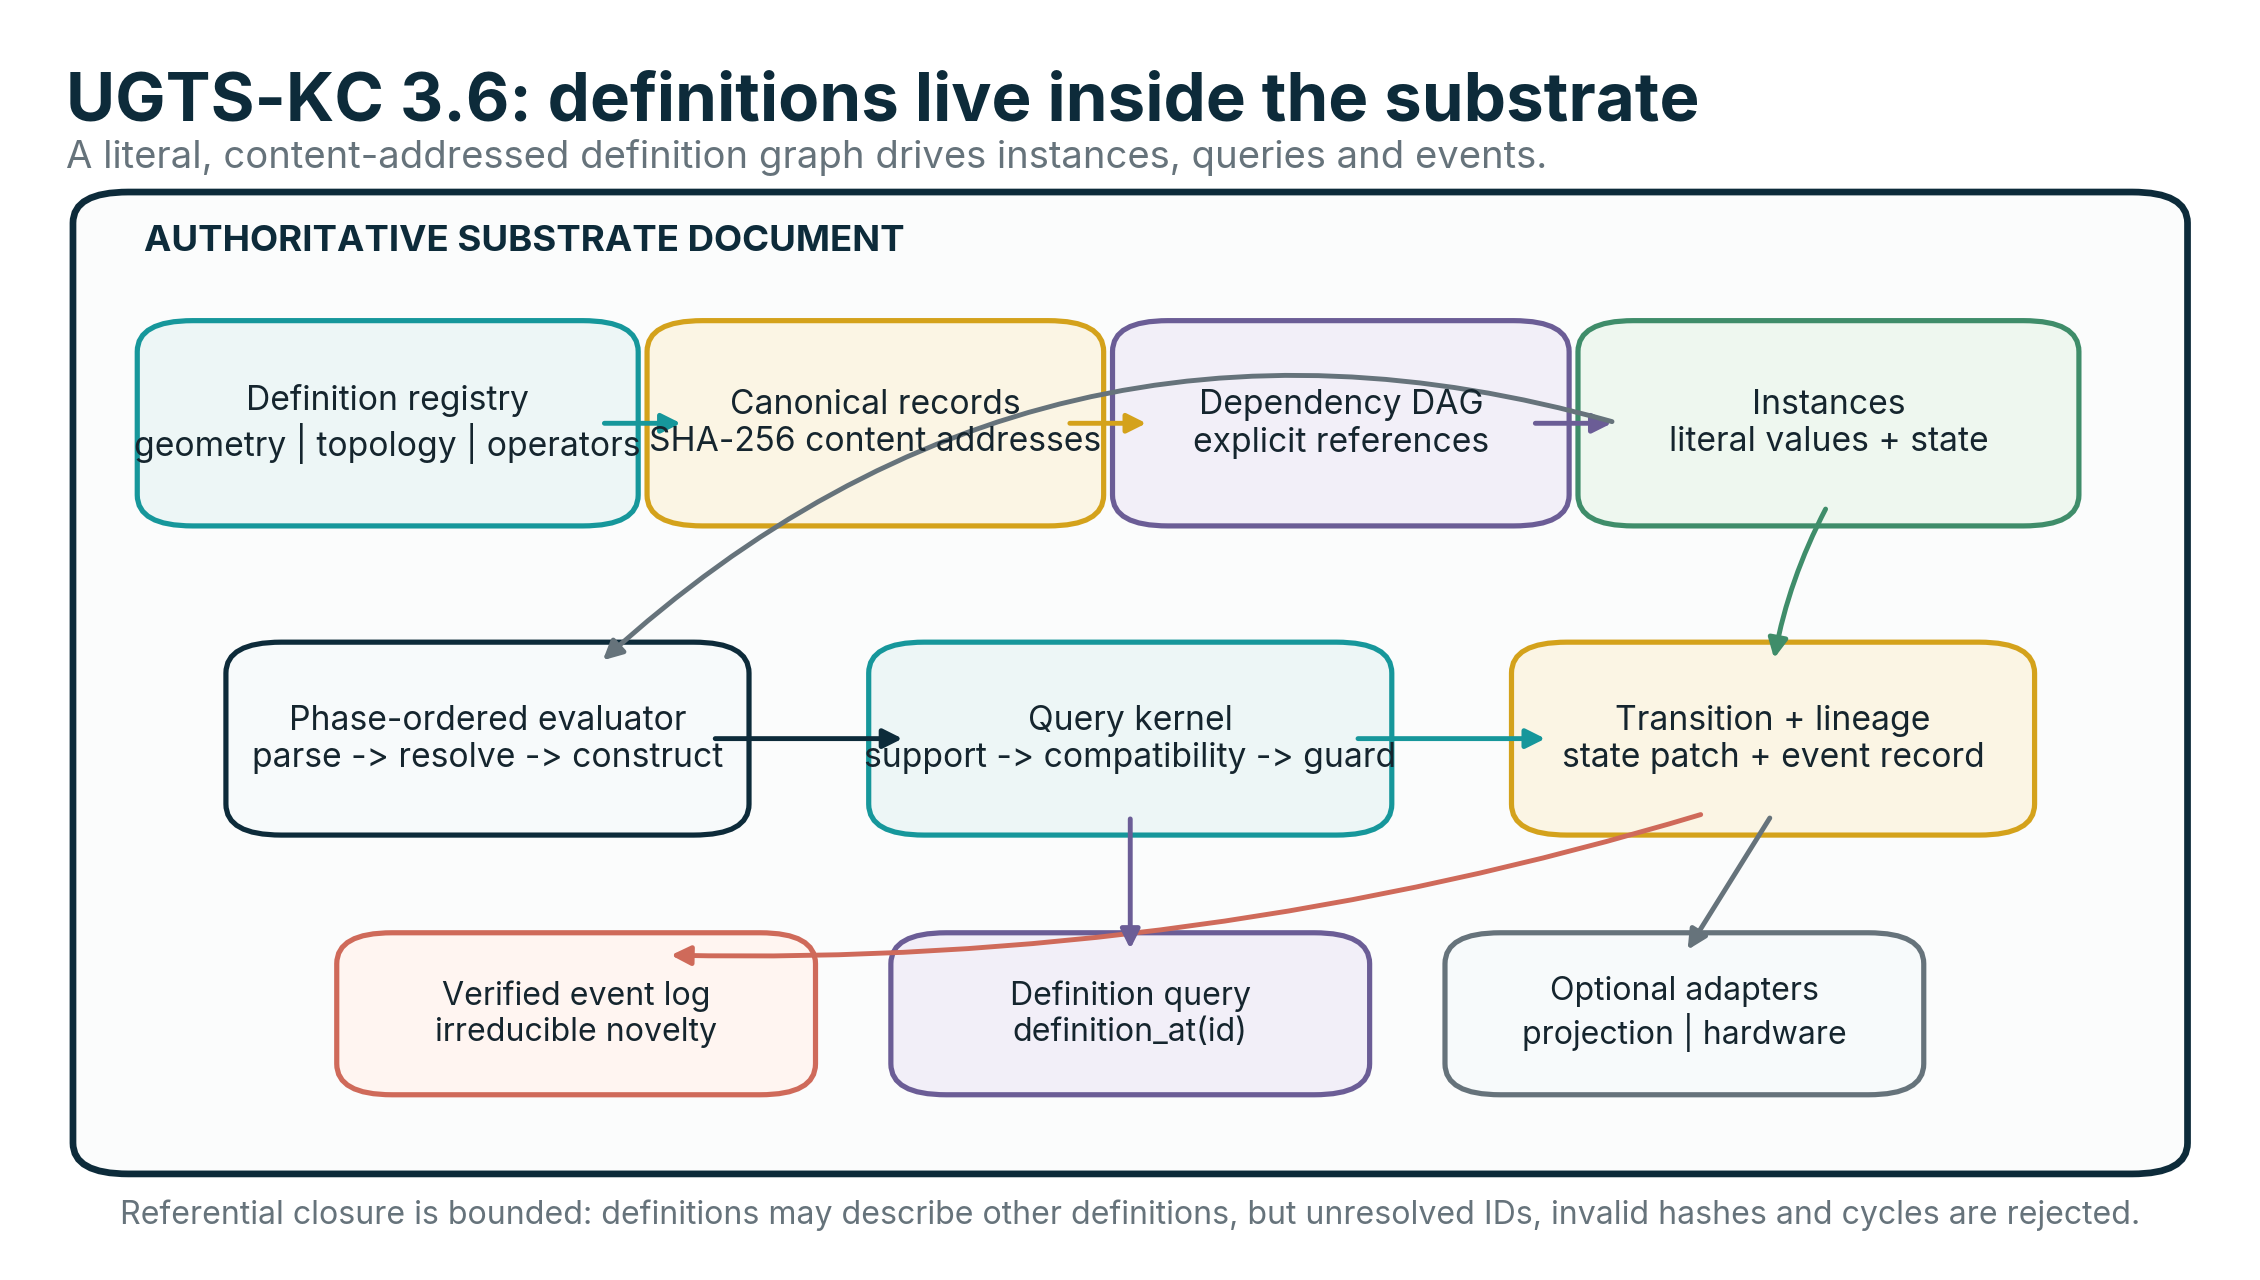
\includegraphics[width=0.96\textwidth]{architecture_referential.png}
\end{center}
\vfill
\begin{tabularx}{\textwidth}{>{\bfseries\sffamily\color{UGTSNavy}}p{4.0cm}>{\RaggedRight\arraybackslash}X}
Version & 3.6.0, 17 August 2026 \\
Requester attribution & Tom Klootwijk; NL200678942; 10-07-1990. Supplied by the requester and not independently verified. \\
Technical scope & 36 v3.6 operators, 20 pattern recipes, 100-entry Dutch number profile, JSON Schema, literal example substrate, dependency-free Python runtime and 36 passing tests. \\
Evidence rule & Source-derived and engineering material remain distinct from corrections and rejections. \\
\end{tabularx}
\end{titlepage}

\pagenumbering{roman}
\section*{Abstract}
The version 3.6 upgrade changes the substrate from a system that merely \emph{uses} geometric and topological definitions into a system that can \emph{carry, resolve and verify those definitions inside itself}. A definition is now a first-class substrate node with a stable ID, typed domain and codomain, explicit dependencies, evaluation phase, provenance class and canonical SHA-256 content address. Instances reference definitions; pipelines reference operator definitions; queries may inspect both state and the definitions that produced it.

The attached Dutch-number dialogue contributes several reusable structures after unrelated subject matter and unsupported extrapolation are removed: radix carry thresholds, active-bit filtering, a chosen count-to-simplex embedding, Pascal parity, local log-polar addressing, one-bit masks, implicit boundaries and hinge language. The central new inference is a clean Dutch number-order calculus. Decimal place order and Dutch spoken order are represented as separate charts. Regular teens place a unit root before \emph{tien}; non-multiple tens from 21 through 99 use \emph{unit + en + tens}. The conjunction \emph{en} is treated as a connector hinge: it has no decimal place magnitude, yet it is structurally necessary in the spoken graph.

The package implements a bounded 0--99 Dutch profile, compares pronunciation-pulse counts with binary Hamming weight without claiming numeric identity, and embeds any declared pulse count as a point, segment or regular polygon. For 19, the decimal value remains 19; binary \code{10011} has three active bits; the shipped profile segments \emph{negentien} as \emph{ne | gen | tien}; and three declared pulses may be embedded as a triangle. The equality is explicitly a feature-count coincidence, not a law connecting language, arithmetic and physics.

\begin{decisionbox}
UGTS-KC 3.6 is a literal referential state-and-event substrate. Its authoritative objects are typed definitions, instances, relations, supports, compatibility gates, hinges, events, transitions and lineage. Rendering, physical devices and narrative associations remain optional downstream uses and cannot redefine the mathematical core.
\end{decisionbox}

\tableofcontents
\clearpage
\pagenumbering{arabic}

\section{Version 3.6 decision and scope}

\subsection{What changed}
The earlier supplied reports already establish the mature query-first sequence: finite grammar, typed state, local support, compatibility, relation guard, earliest valid event, transition and lineage. They also insist that one-bit values remain narrow flags and that topology is an explicit routing or gluing rule rather than material magic. UGTS-KC 3.6 retains those boundaries and adds six architectural commitments:

\begin{enumerate}
\item \textbf{Definitions are substrate data.} Geometry, topology, phonetic profiles, hinges, schedules and operators are stored in the same literal document as instances and pipelines.
\item \textbf{References are resolvable.} Every dependency and \code{definition_ref} must resolve to a unique definition ID.
\item \textbf{Definitions are content-addressed.} Canonical JSON records are hashed, excluding the hash field itself.
\item \textbf{Operation order is explicit.} A normative ten-phase schedule removes ambiguity about which transformations occur first.
\item \textbf{Dutch number morphology is typed.} Numeric place order, orthography, pronunciation-like segments, morphemes, spoken order and hinge nodes are separate fields.
\item \textbf{Cross-domain matches remain metadata.} Equal counts may seed patterns, but do not become numeric identity or physical causation.
\end{enumerate}

\subsection{Deliverables}
The accompanying ZIP contains:

\begin{itemize}
\item this PDF and its editable LaTeX source;
\item a JSON Schema and a fully literal example substrate with content hashes;
\item 36 v3.6 operator definitions and 20 reusable pattern recipes in CSV and JSON;
\item a bounded Dutch 0--99 profile in CSV and JSON, plus a pulse-match extract;
\item dependency-free Python modules for canonicalization, geometry, topology, Dutch number profiles, definition loading and pipeline execution;
\item original diagrams, a reproducible demonstration and 36 passing unit tests;
\item privacy-safe source notes, SHA-256 source hashes and package checksums.
\end{itemize}

\begin{boundarybox}
The v3.6 document is a technical specification and reference implementation. It is not independent scientific validation, a patent grant, proof of authorship priority, a physical-device benchmark or evidence that numerical coincidences establish hidden causal laws.
\end{boundarybox}

\section{Evidence discipline and source analysis}

\subsection{Admission rule}
A motif enters the technical core only if it can be expressed as at least one of the following: a typed literal, coordinate map, geometric definition, topology/gluing map, hinge, support predicate, compatibility predicate, relation guard, event solver, transition, invariant, lineage rule, bounded grammar, evaluation schedule or measurable error/resource quantity.

The package uses the following dispositions:

\begin{center}
\begin{tabularx}{0.95\textwidth}{>{\bfseries}p{2.5cm}X}
\toprule
RETAIN & Exact or directly reusable operator. \\
ENGINEERING & New typed implementation or structural inference that preserves a source motif. \\
CORRECTED & Useful mechanism kept after an explicit mathematical, dimensional or semantic correction. \\
BOUNDED & Valid only under a declared language profile, schema, relation family, tolerance or finite range. \\
DEMOTE & Analogy or research prompt, not a core operator. \\
REJECT & Unsupported totalizing, physical or causal claim. \\
\bottomrule
\end{tabularx}
\end{center}

\subsection{Hidden tricks extracted from the attached documents}
\renewcommand{\arraystretch}{1.15}
\begin{longtable}{>{\raggedright\arraybackslash}p{3.3cm}>{\raggedright\arraybackslash}p{6.0cm}>{\raggedright\arraybackslash}p{6.2cm}}
\toprule
\textbf{Motif} & \textbf{Reusable mechanism} & \textbf{Boundary or correction} \\
\midrule
\endfirsthead
\toprule
\textbf{Motif} & \textbf{Reusable mechanism} & \textbf{Boundary or correction} \\
\midrule
\endhead
Radix carry threshold & Digit-count changes at $b^k$; use powers of the radix as scale events or shell indices. & The threshold is an exact number-system fact, not proof that physical geometry is inherently binary or decimal. \\
Active bits and ``zero as silence'' & Extract set-bit positions and Hamming weight as a sparse feature projection. & Deleting zeros from a displayed feature string never changes the numeric value. \\
Three active units & Map a declared count of three to three non-collinear vertices. & The triangle is a chosen embedding; three is not automatically a geometric triangle in every domain. \\
Pascal parity & Use $\binom{n}{k}\bmod 2$ as a deterministic Sierpiński occupancy test. & With zero-based rows, $2^m-1$ rows are all odd; generic $2^m$ rows are not. \\
Combination count & $\binom{5}{3}=10$ counts placements of three selected positions among five. & The result is not a causal proof of the decimal 9--10 threshold. \\
Log-polar chart & $\rho=\ln(r/r_0)$ converts radial scaling into additive displacement. & The origin remains singular and requires an explicit core chart. \\
One-bit jitter & A bit may select a deterministic dither threshold, route, latch or mask. & It redistributes error; it does not guarantee perfect anti-aliasing, infinite resolution or zero cost. \\
SDF language & Use an implicit field sign and promote $f=0$ to an event relation. & A generic implicit field is not automatically an exact signed-distance function. \\
Cut/unroll glyph morph & Edit a boundary graph by cutting an edge, releasing an endpoint and interpolating curve controls. & Intermediate fields may lose exact-distance status; topology state changes at an explicit event. \\
Parity hinge & A one-bit state selects one of two declared maps. & The bit is not continuous state, geometry, uncertainty or identity. \\
Double-vacuum motif & Same coordinate, different sheet/phase/orientation may fail compatibility. & Co-location is necessary but not sufficient for coupling. \\
Möbius/Klein motifs & Implement quotient/gluing maps with explicit orientation and sheet transport. & No physical self-intersection, self-assembly or energy creation follows. \\
Hourglass/pinch motif & Four finite sectors meet at a guarded routing locus. & The pinch is an event/router, not a destructive singularity. \\
Self-reference and strange loops & Represent definitions and cycles as a graph with budgets and cycle policy. & Undeclared recursion and unbounded self-generation are rejected. \\
Dutch number order & Treat decimal place order and spoken morphological order as separate charts connected by a typed hinge map. & This is a language-profile transform, not changed arithmetic. \\
\bottomrule
\end{longtable}

\begin{correctionbox}
The new dialogue contains several persuasive but unsupported escalations: generic SDFs described as exact distances, one-bit jitter described as eliminating aliasing, log-polar coordinates described as infinite storage-free resolution, personal numbers treated as physical invariants, and historical/geological facts inferred from decimal patterns. UGTS-KC 3.6 keeps the reusable operators and rejects those conclusions.
\end{correctionbox}

\section{Literal referential substrate architecture}

\subsection{World object}
The v3.6 world is defined as
\[
\mathcal{W}_{3.6}=(\mathcal{D},\mathcal{X},\mathcal{G},\mathcal{R},\mathcal{S},\mathcal{C},\mathcal{H},\mathcal{E},\mathcal{T},\mathcal{I},\mathcal{L},\mathcal{P}),
\]
where $\mathcal{D}$ is the in-substrate definition registry, $\mathcal{X}$ instances, $\mathcal{G}$ bounded grammar, $\mathcal{R}$ relations/fields, $\mathcal{S}$ support predicates, $\mathcal{C}$ compatibility, $\mathcal{H}$ hinges, $\mathcal{E}$ events, $\mathcal{T}$ transitions, $\mathcal{I}$ invariants, $\mathcal{L}$ lineage and external novelty log, and $\mathcal{P}$ phase-ordered pipelines.

The architectural change is the explicit $\mathcal{D}$ component. A substrate no longer depends on prose outside the data to explain what \code{sphere}, \code{nl_number_lexeme}, \code{mobius_quotient} or \code{guard} means. Those definitions are themselves queryable records.

\subsection{Definition record}
\begin{definitionbox}
A literal definition node is
\[
d=(id,kind,A,B,\theta,Dep,phase,cap,inv,prov,h),
\]
with domain $A$, codomain $B$, literal parameters $\theta$, dependency IDs $Dep$, evaluation phase, capabilities, invariants, provenance and content hash $h$.
\[
h=\operatorname{SHA256}(\operatorname{canonicalJSON}(d\setminus\{h\})).
\]
The hash is verification metadata, not a cryptographic ownership claim.
\end{definitionbox}

An instance is
\[
x=(id,definition\_ref,literal,state),
\]
and a pipeline is an ordered sequence of definition IDs. Referential closure requires every reference to resolve, every content hash to verify and the dependency graph to admit a topological order.

\begin{figure}[H]
\centering
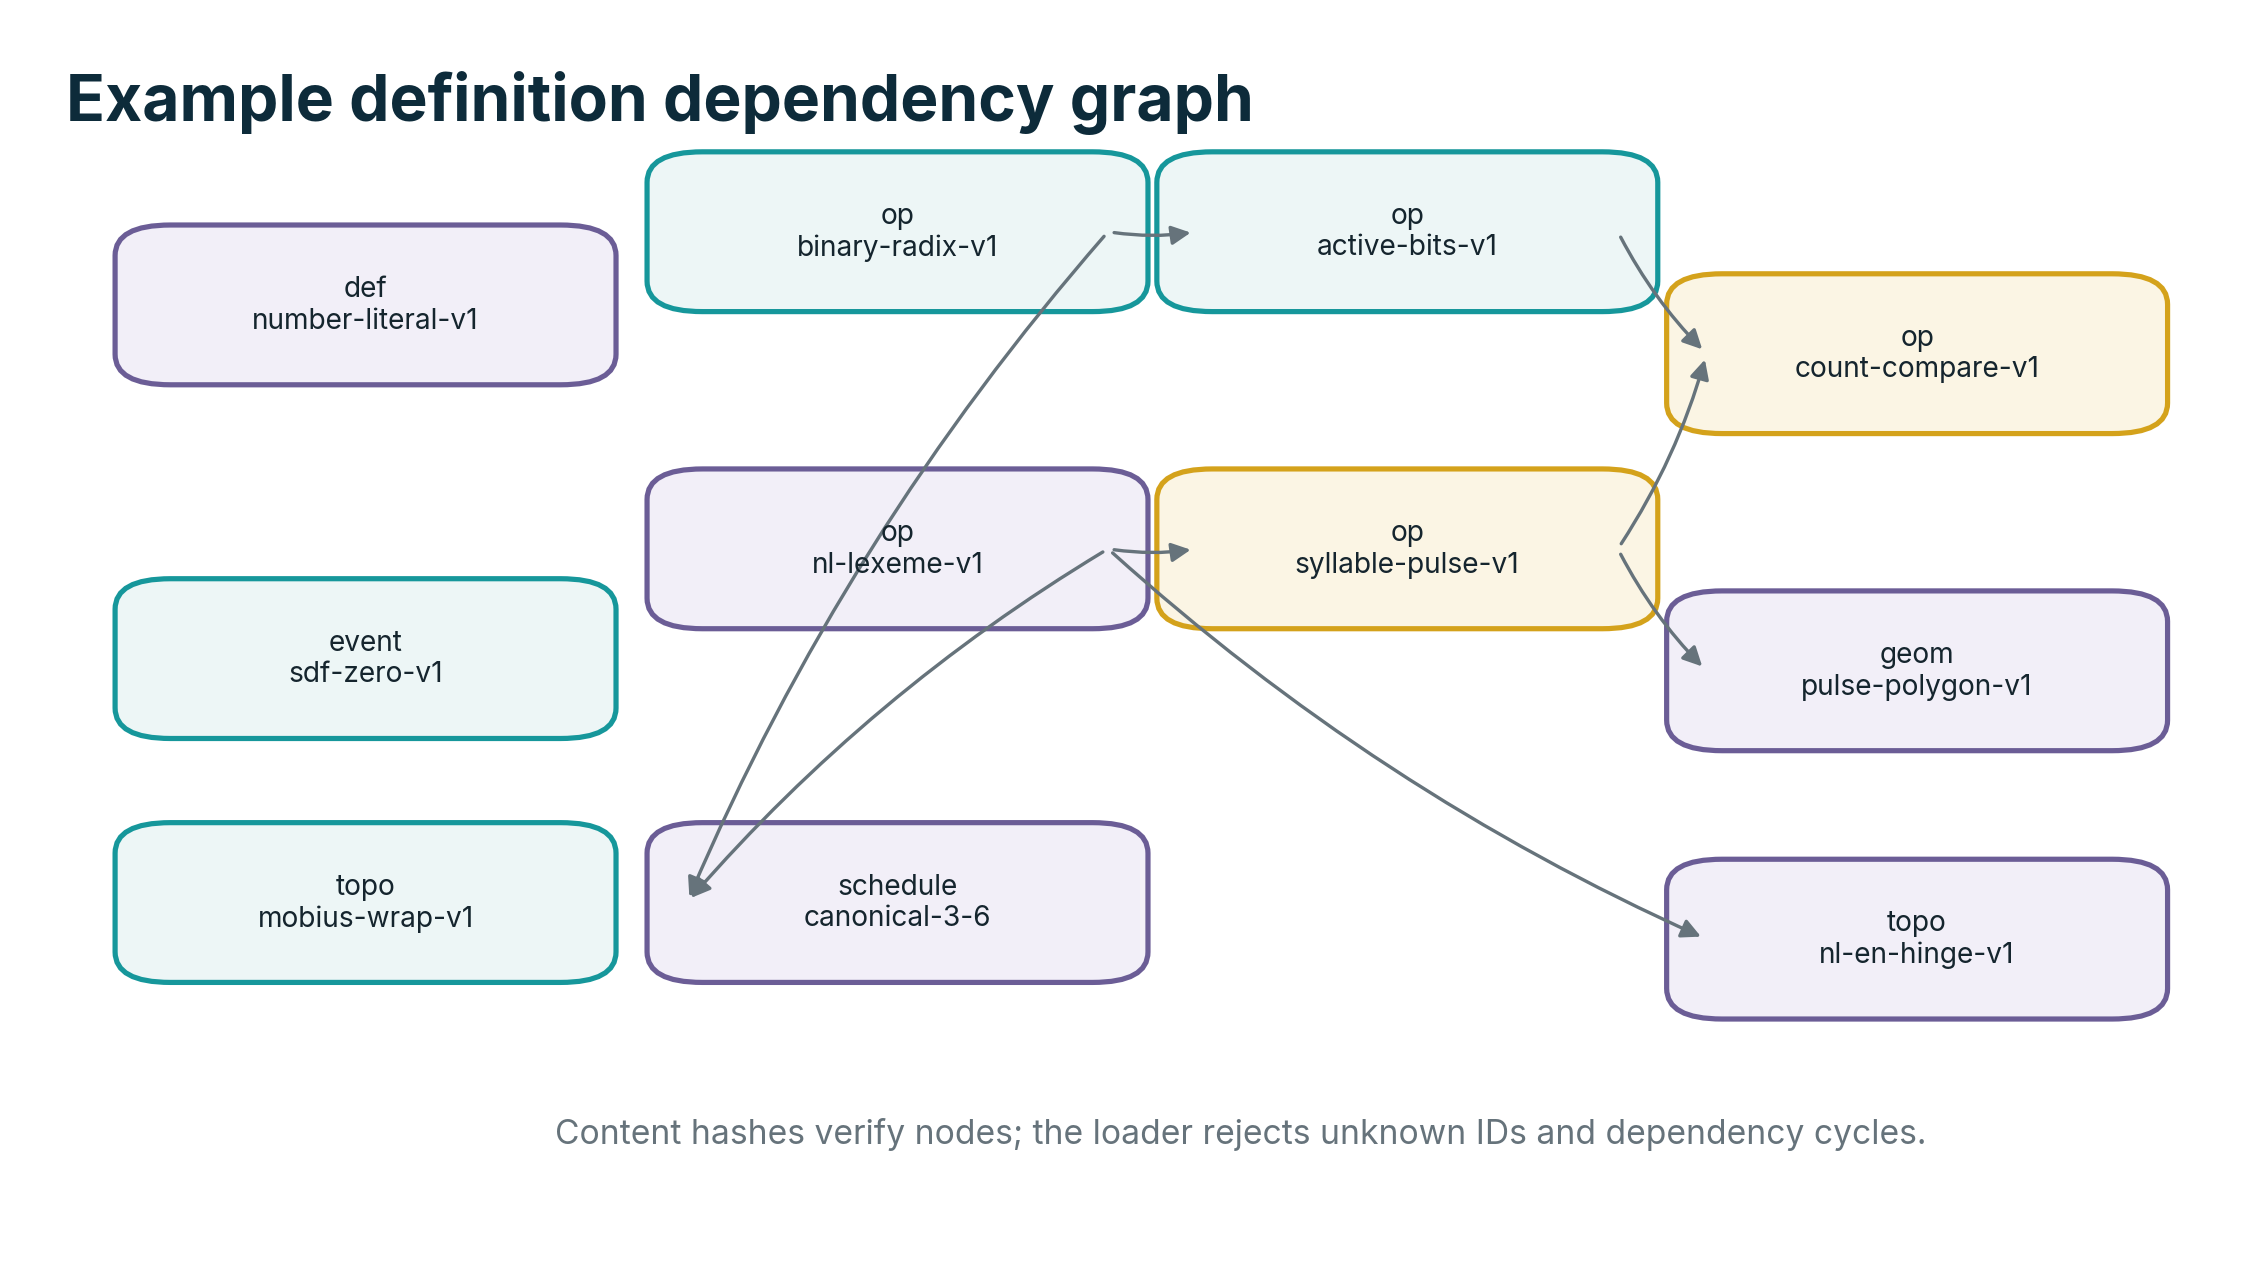
\includegraphics[width=0.94\textwidth]{definition_graph.png}
\caption{The shipped example contains literal definition nodes and explicit dependency edges.}
\end{figure}

\subsection{Definition queries}
The minimum referential API is:
\begin{itemize}
\item \code{definition_at(id)} -- return the exact typed record and content hash;
\item \code{definition_order()} -- return a deterministic dependency order;
\item \code{instances_of(definition_id)} -- enumerate literal uses;
\item \code{trace(pipeline, instance)} -- return ordered definition IDs, operator kinds and typed outputs;
\item \code{verify_definition(id)} -- recompute the canonical content hash;
\item \code{explain_reference(id)} -- return dependencies, provenance and evaluation phase.
\end{itemize}

\section{Geometry definition calculus}

\subsection{Parametric and implicit forms}
A parametric geometric definition has the form
\[
\gamma:U\rightarrow\mathbb{R}^n,\qquad u\mapsto\gamma(u),
\]
with a declared interval, regularity and frame policy. An implicit definition is
\[
f:\mathbb{R}^n\rightarrow\mathbb{R},\qquad f(x)<0\text{ inside},\quad f(x)=0\text{ boundary},\quad f(x)>0\text{ outside}.
\]
Exact signed-distance status is a capability, not a synonym for ``implicit.'' CSG sign composition remains useful:
\[
f_{A\cup B}=\min(f_A,f_B),\qquad f_{A\cap B}=\max(f_A,f_B),\qquad f_{A\setminus B}=\max(f_A,-f_B).
\]
These formulas preserve inside/outside sign semantics, but smooth blends and generic morphs need not remain exact distances.

\subsection{Radix shells and log-polar charts}
For radix $b\ge 2$, digit-count transitions occur at $b^k$. The exact digit count is
\[
\operatorname{digits}_b(n)=\begin{cases}1,&n=0,\\ \lfloor\log_b n\rfloor+1,&n>0.\end{cases}
\]
UGTS 3.6 may map those thresholds to local shells $[b^k,b^{k+1})$. This is an indexing choice. The local log-polar chart is
\[
\rho=\ln(r/r_0),\qquad \theta=\operatorname{atan2}(y,x),
\]
with a mandatory \code{core=true} flag when $r<\varepsilon$.

\subsection{Pulse geometry}
For a declared pulse sequence of length $m$, the reference embedding is
\[
p_j=r\bigl(\cos(\phi+2\pi j/m),\sin(\phi+2\pi j/m)\bigr),\quad j=0,\ldots,m-1.
\]
The special cases are one pulse $\mapsto$ one point, two pulses $\mapsto$ a segment and three pulses $\mapsto$ a triangle. Four or more pulses yield a regular polygon. Pulse identity and source positions remain metadata; geometry never replaces them.

\section{Topology and hinge calculus}

\subsection{Topology as explicit gluing}
A quotient/gluing definition names entry and exit ports, coordinate transport, orientation transport, optional sheet change and lineage update. A Möbius-style horizontal wrap can be written
\[
(0,y,o)\sim(w,h-y,-o).
\]
The explicit state prevents a projected self-intersection from being mistaken for a physical collision.

\begin{figure}[H]
\centering
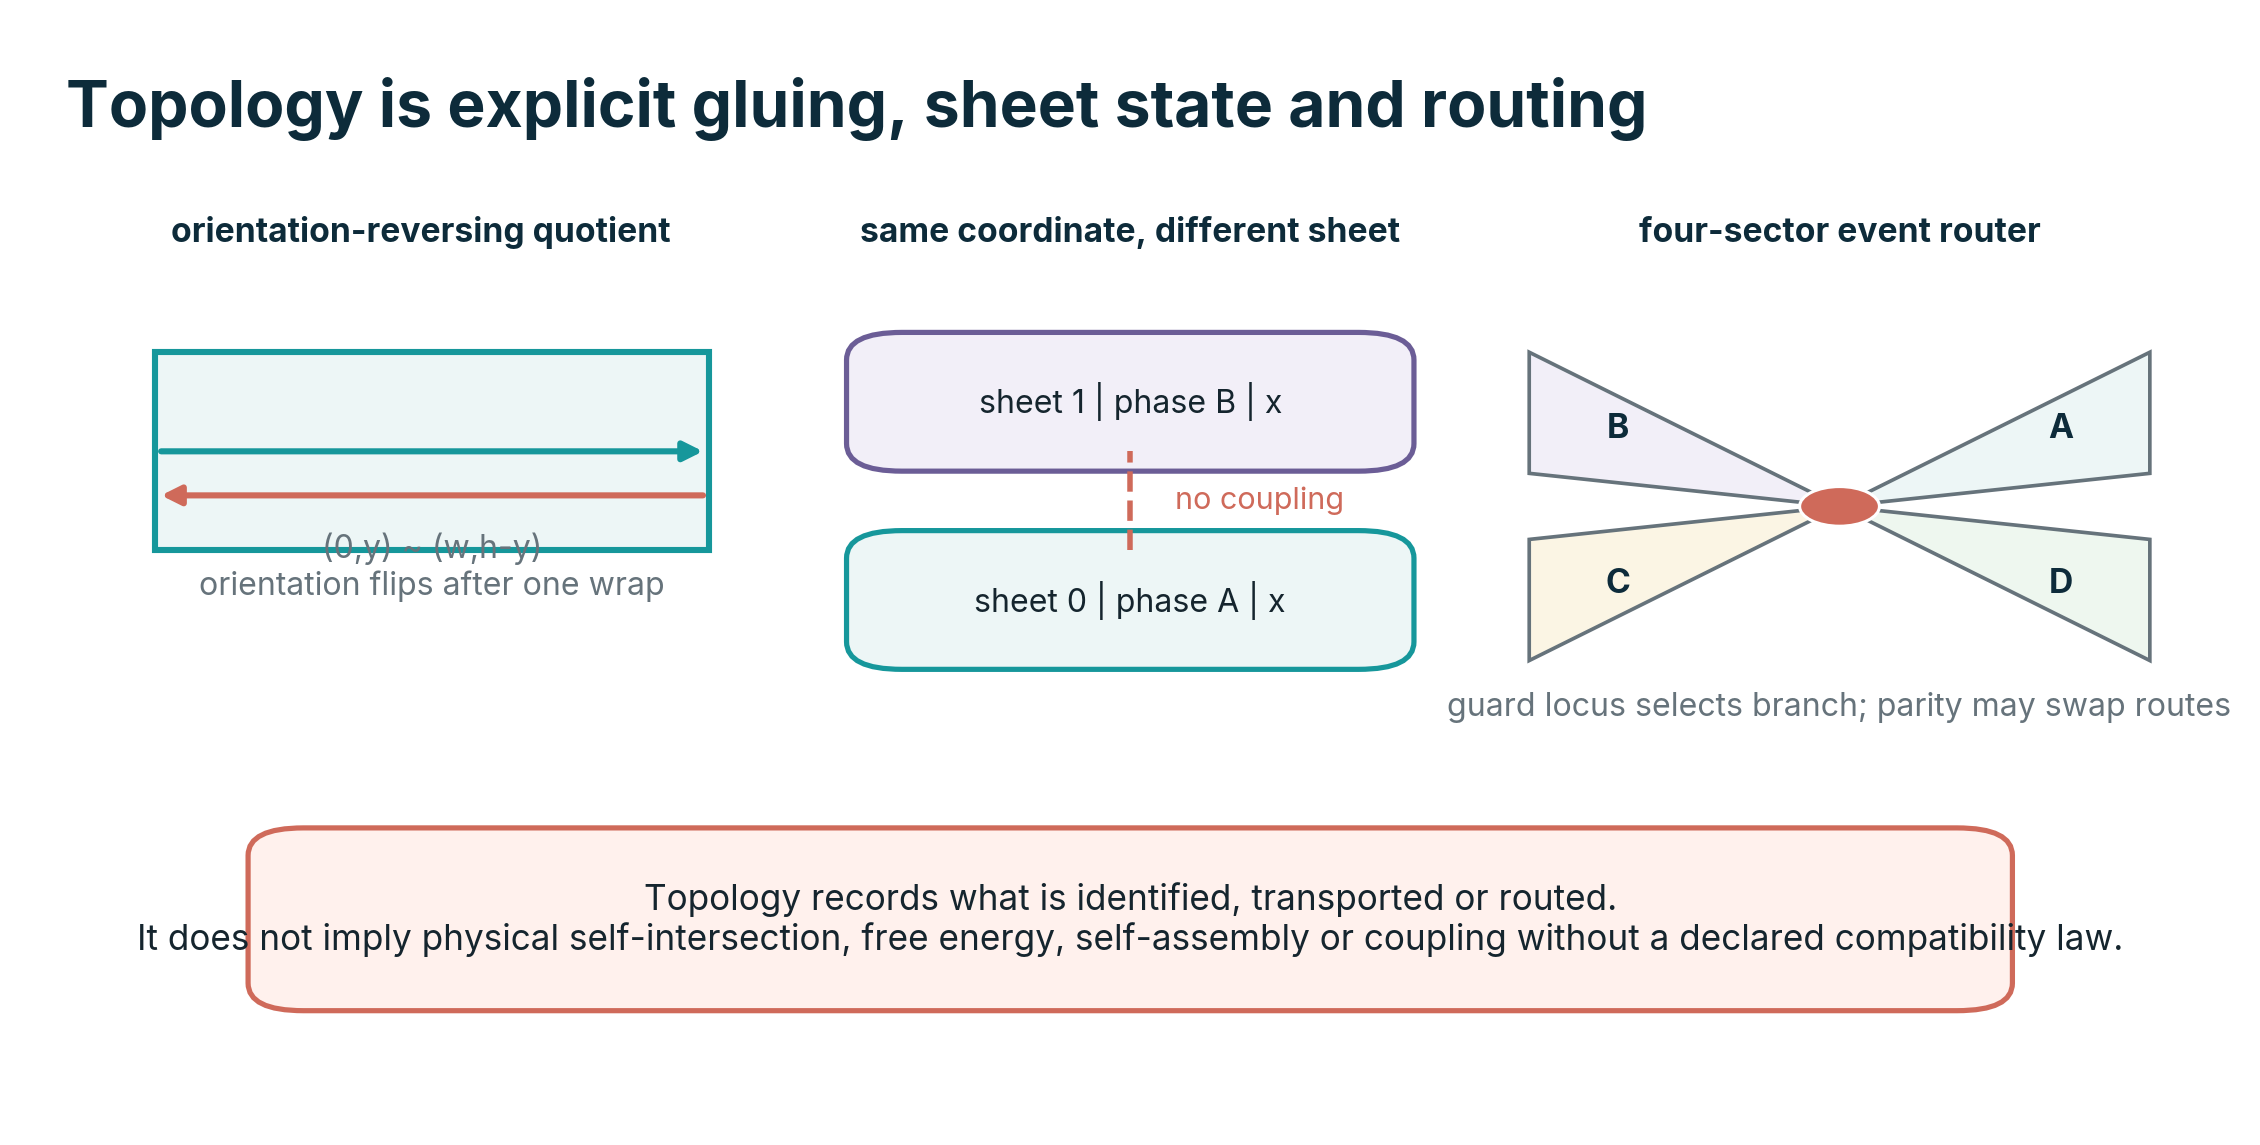
\includegraphics[width=0.95\textwidth]{topology_gluing.png}
\caption{Three distinct topology mechanisms: quotient gluing, compatibility-separated sheets and finite event routing.}
\end{figure}

\subsection{Generic hinge}
\begin{definitionbox}
A hinge is a typed tuple
\[
H=(p,h,M,g,F),
\]
where $p$ is a pivot or connector locus, $h$ the continuous or discrete hinge state, $M_h$ the selected map, $g$ a guard for state change, and $F$ declared invariants or fixed subspaces.
\end{definitionbox}

A continuous planar hinge about pivot $p$ uses
\[
x'(t)=p+R(\theta(t))(x-p).
\]
Its velocity is
\[
\dot{x}'(t)=\dot{\theta}(t)J R(\theta(t))(x-p),\qquad J=\begin{bmatrix}0&-1\\1&0\end{bmatrix}.
\]
A discrete parity hinge selects $M_0$ or $M_1$ only after a guarded event. A connector hinge inserts a graph node that may have zero numeric magnitude but nonzero structural role.

\subsection{Composition order}
Hinge composition is generally non-commutative:
\[
H_2\circ H_1\ne H_1\circ H_2.
\]
For an articulated chain,
\[
T(q)=T_n(q_n)\cdots T_2(q_2)T_1(q_1).
\]
UGTS-KC 3.6 stores that order literally. It does not sort transforms by name or silently commute them.

\begin{figure}[H]
\centering
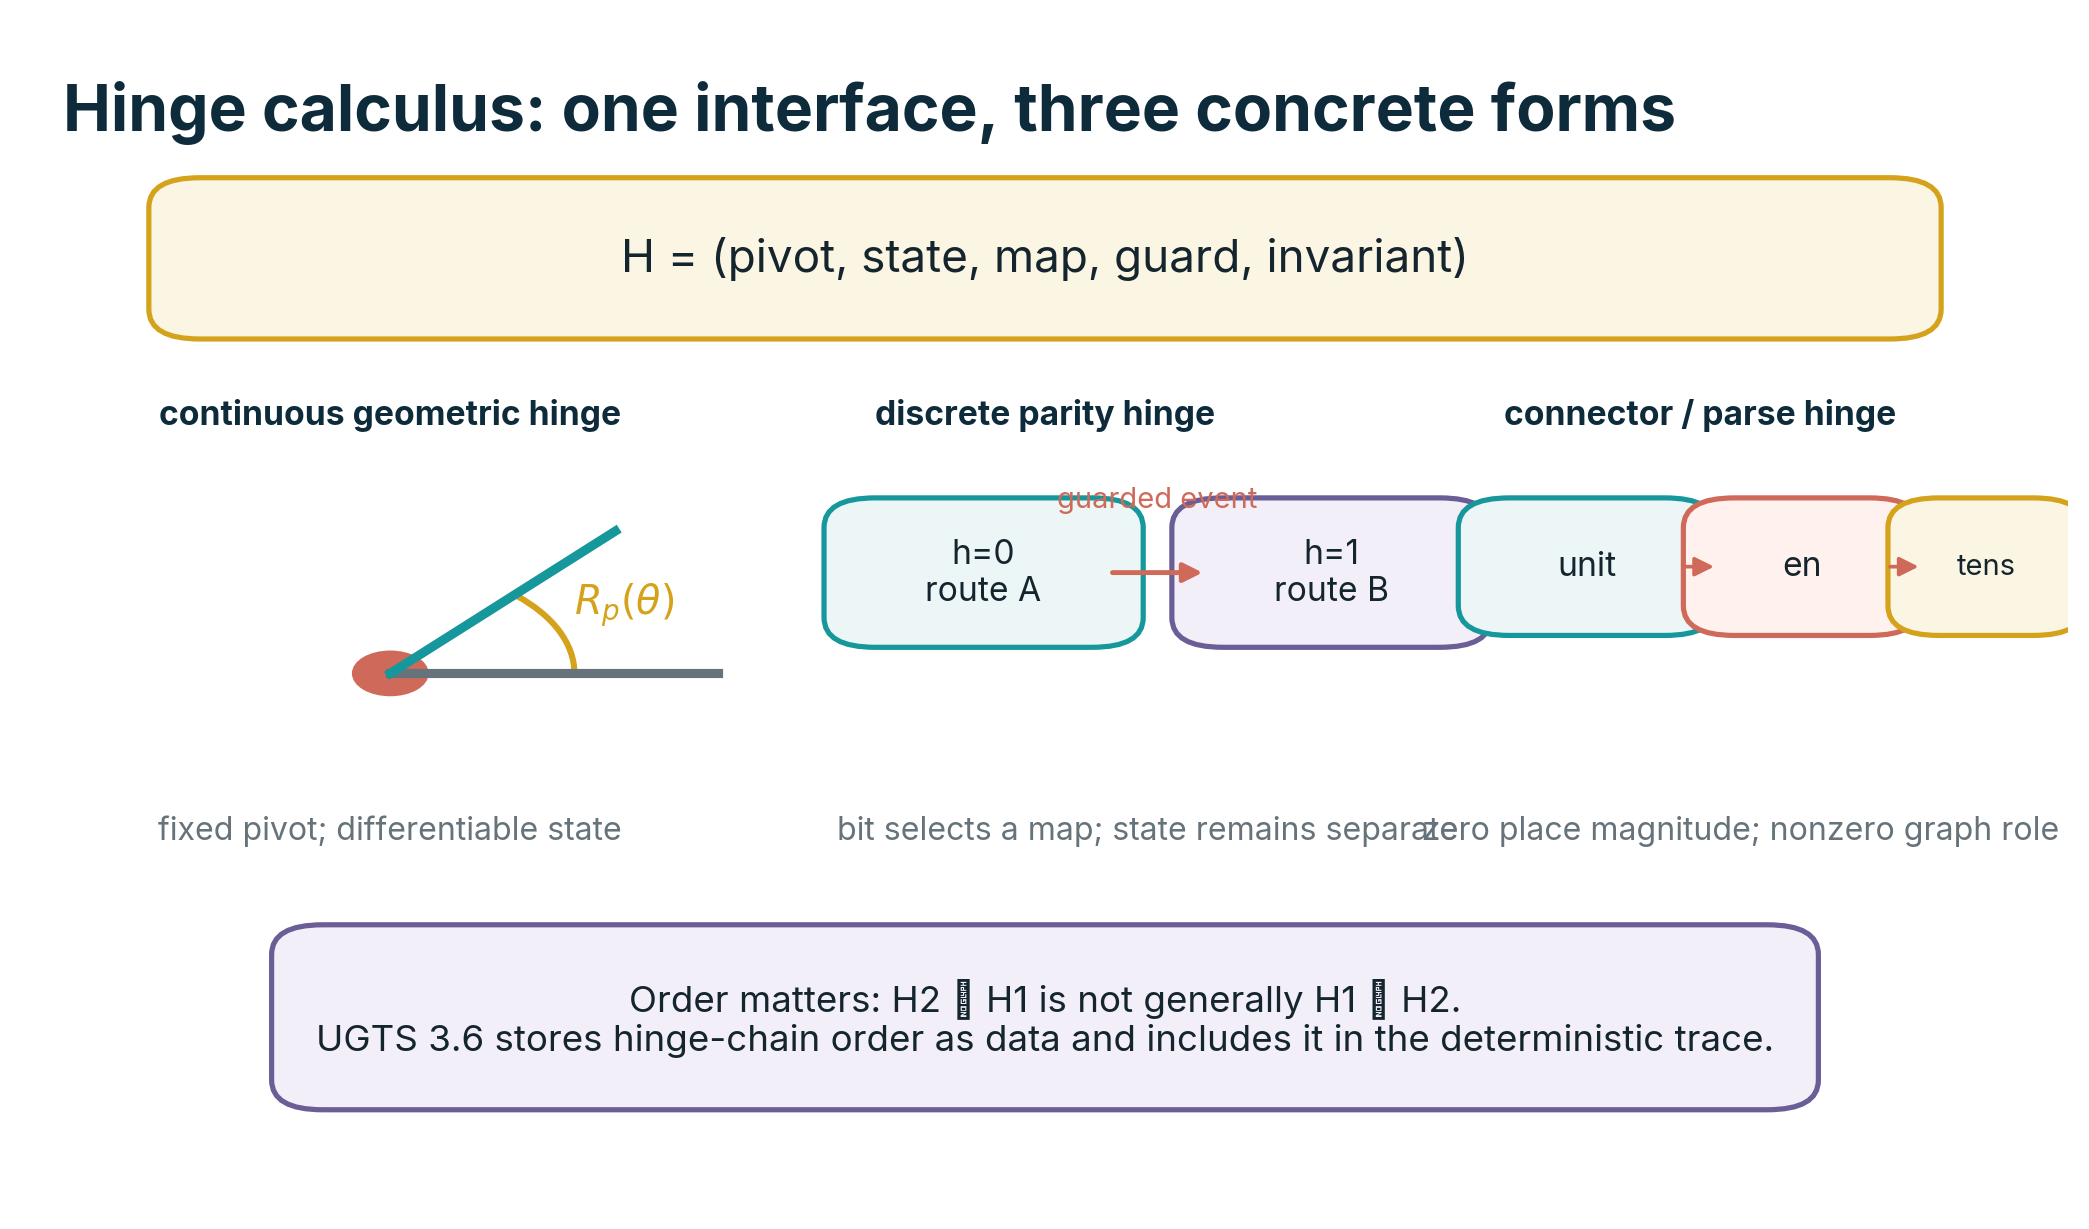
\includegraphics[width=0.92\textwidth]{hinge_calculus.png}
\caption{Continuous rotation, a discrete parity selector and a connector hinge share one typed interface.}
\end{figure}

\section{Dutch phonetic-number calculus}

\subsection{Profile boundary}
The shipped \code{phon:nl-NL-standard-0-99-v1} profile covers integers 0 through 99. It records standard orthography, pronunciation-like segments, morphemes, decimal place order, spoken semantic order, hinge kind, binary spelling and Hamming weight. The segment list is a versioned engineering profile, not an IPA transcription or a claim about every dialect.

\subsection{Place order and spoken order}
For a non-multiple ten $n=10t+u$ with $t\in\{2,\ldots,9\}$ and $u\in\{1,\ldots,9\}$, decimal place semantics are
\[
P(n)=(10t,u),
\]
while the standard Dutch spoken graph is represented as
\[
S_{nl}(n)=(u,\text{en},10t).
\]
The connector hinge is therefore
\[
H_{en}(10t,u)=(u,\text{en},10t).
\]
The invariant is numeric value:
\[
\operatorname{value}(P(n))=\operatorname{value}(S_{nl}(n))=n.
\]
The node \emph{en} has no place value, yet its omission would change the declared spoken graph.

For regular teens 13 through 19, place semantics are $(10,u)$ while morphology places the unit root before the suffix \emph{tien}. Eleven and twelve remain explicit irregular lexemes.

\begin{figure}[H]
\centering
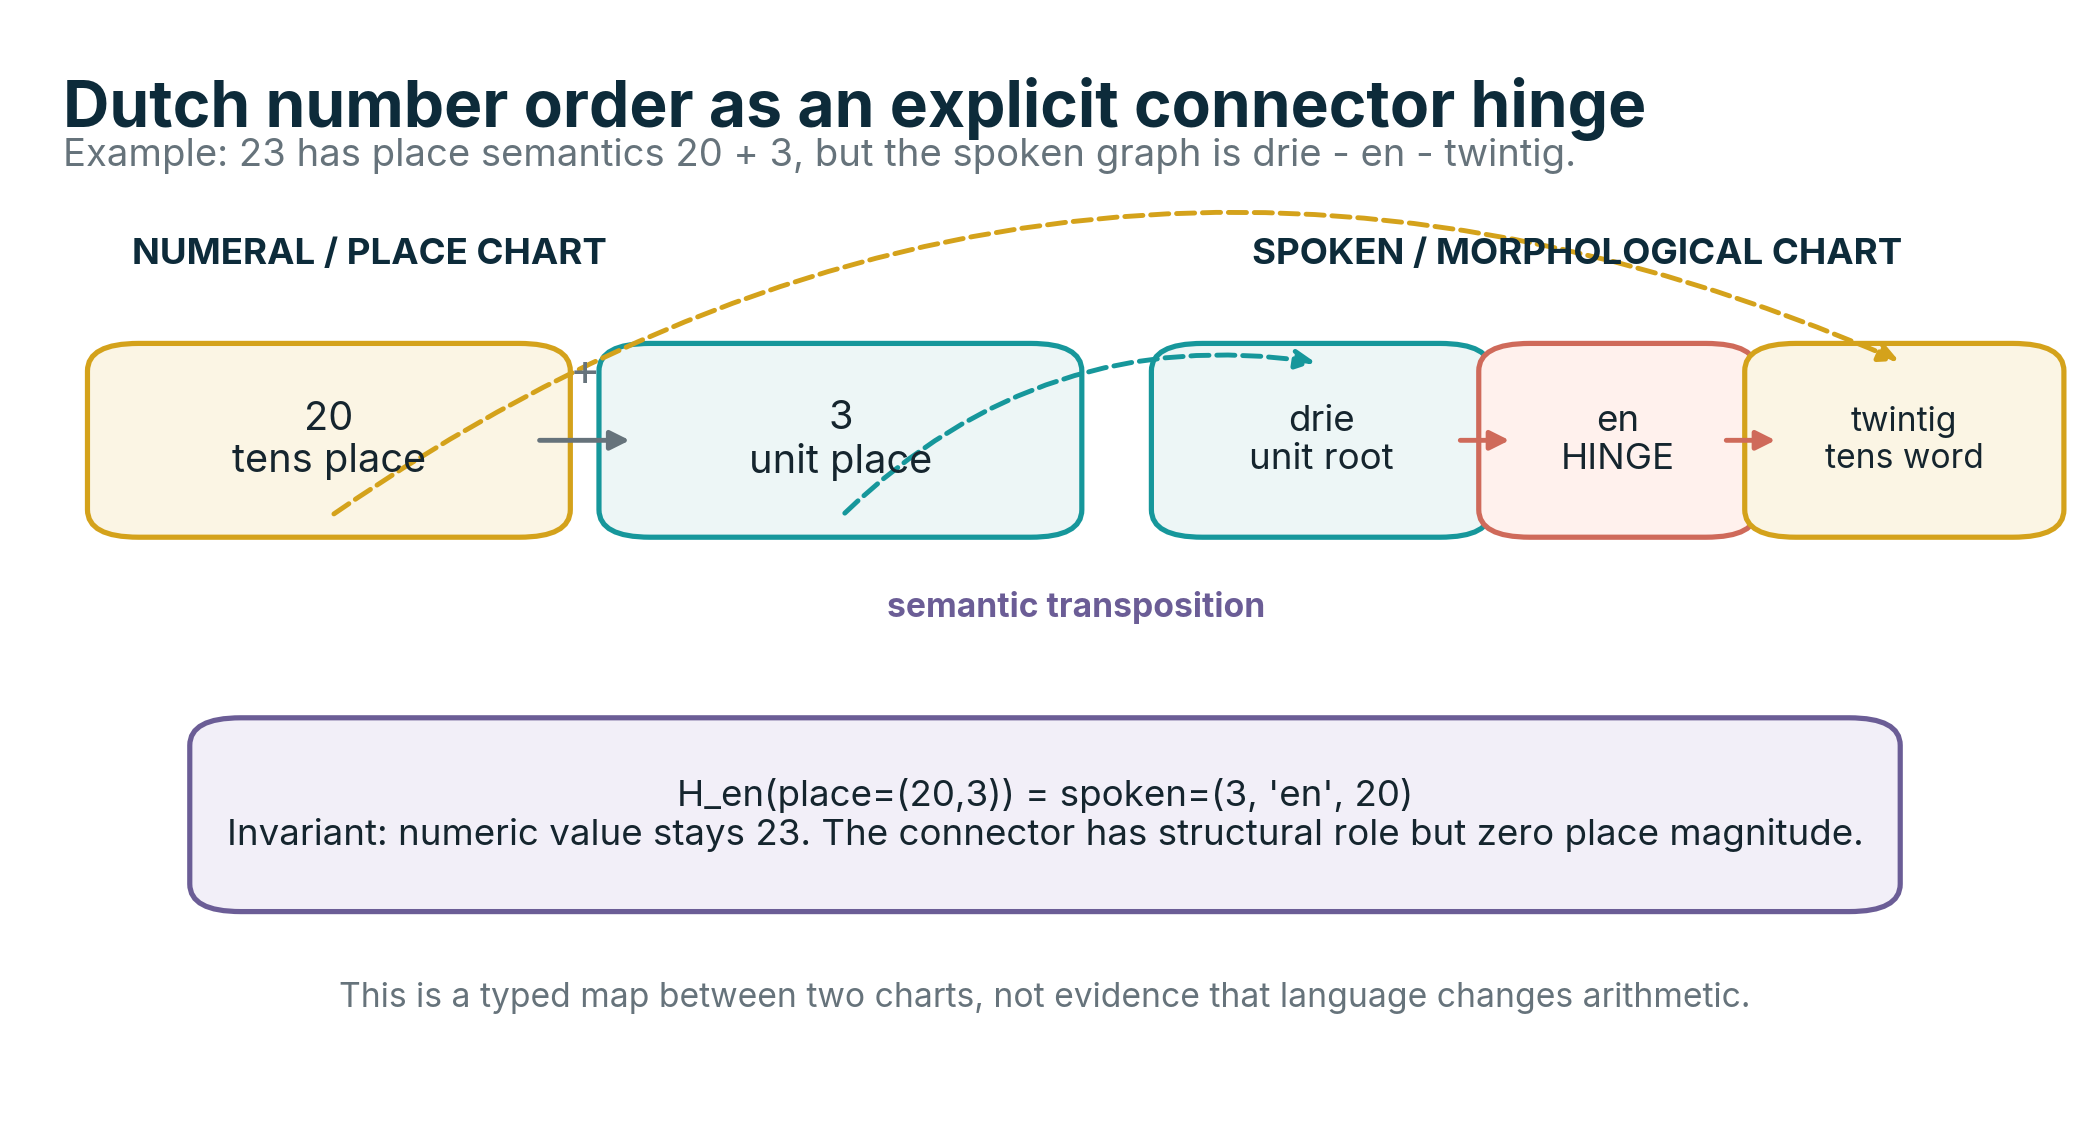
\includegraphics[width=0.92\textwidth]{dutch_hinge_23.png}
\caption{The Dutch \emph{en} connector is modeled as a structural hinge between place and spoken charts.}
\end{figure}

\subsection{Syllable-pulse operator}
Let the profile return segments
\[
\Sigma_{nl}(n)=(s_1,\ldots,s_m).
\]
The pulse projection is
\[
\Pi_{phon}(n)=(1,\ldots,1)\in\{1\}^m,
\]
so $|\Pi_{phon}(n)|=m$. Independently, the binary active set is
\[
A_2(n)=\{k\mid \operatorname{bit}_k(n)=1\},\qquad \operatorname{popcount}(n)=|A_2(n)|.
\]
The comparison flag is
\[
M(n)=\mathbf{1}\bigl[|\Pi_{phon}(n)|=|A_2(n)|\bigr].
\]
The codomain of $M$ is metadata. It is not a rewrite of $n$.

\subsection{Worked example: 19}
The shipped trace records:
\begin{align*}
\operatorname{value} &= 19,\\
\operatorname{binary}_2(19) &= 10011,\\
A_2(19)&=\{0,1,4\},\quad |A_2(19)|=3,\\
\Sigma_{nl}(19)&=(\text{ne},\text{gen},\text{tien}),\quad |\Sigma_{nl}(19)|=3,\\
M(19)&=1\quad\text{with semantics ``equal feature counts; no numeric identity.''}
\end{align*}
A three-vertex pulse embedding yields a triangle. The positions 0, 1 and 4 remain available as source metadata; they are not discarded.

\begin{figure}[H]
\centering
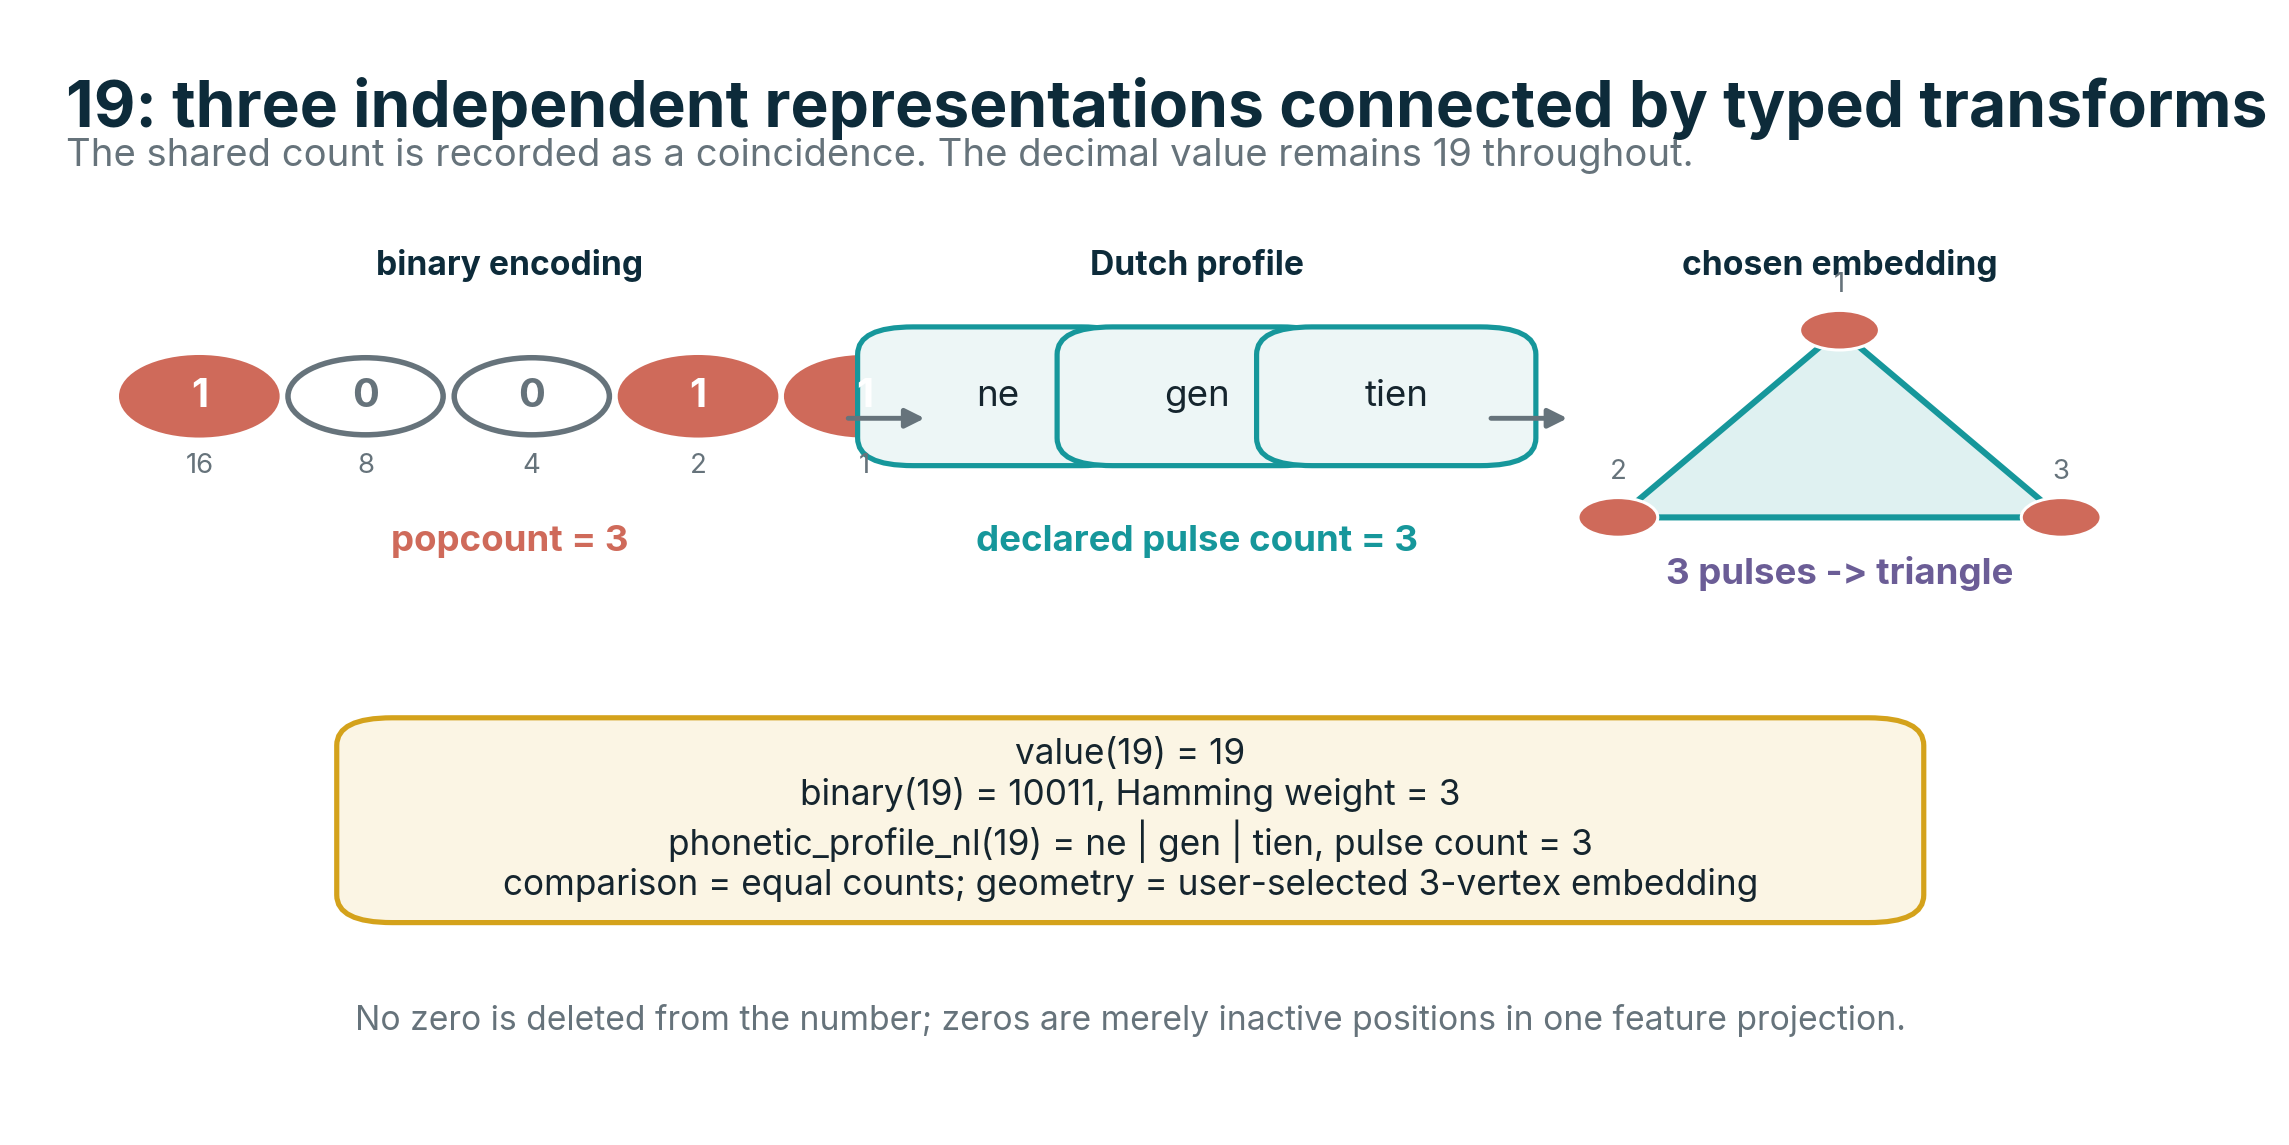
\includegraphics[width=0.95\textwidth]{number19_typed_pipeline.png}
\caption{The three-count connection is explicit, typed and bounded.}
\end{figure}

\subsection{Bounded atlas result}
Across the shipped 0--99 profile, 28 values have equal pronunciation-pulse count and binary popcount. That result depends on this exact lexicon and segmentation profile. It is useful as a pattern-search dataset, not as a universal law of Dutch or binary arithmetic.

\begin{figure}[H]
\centering
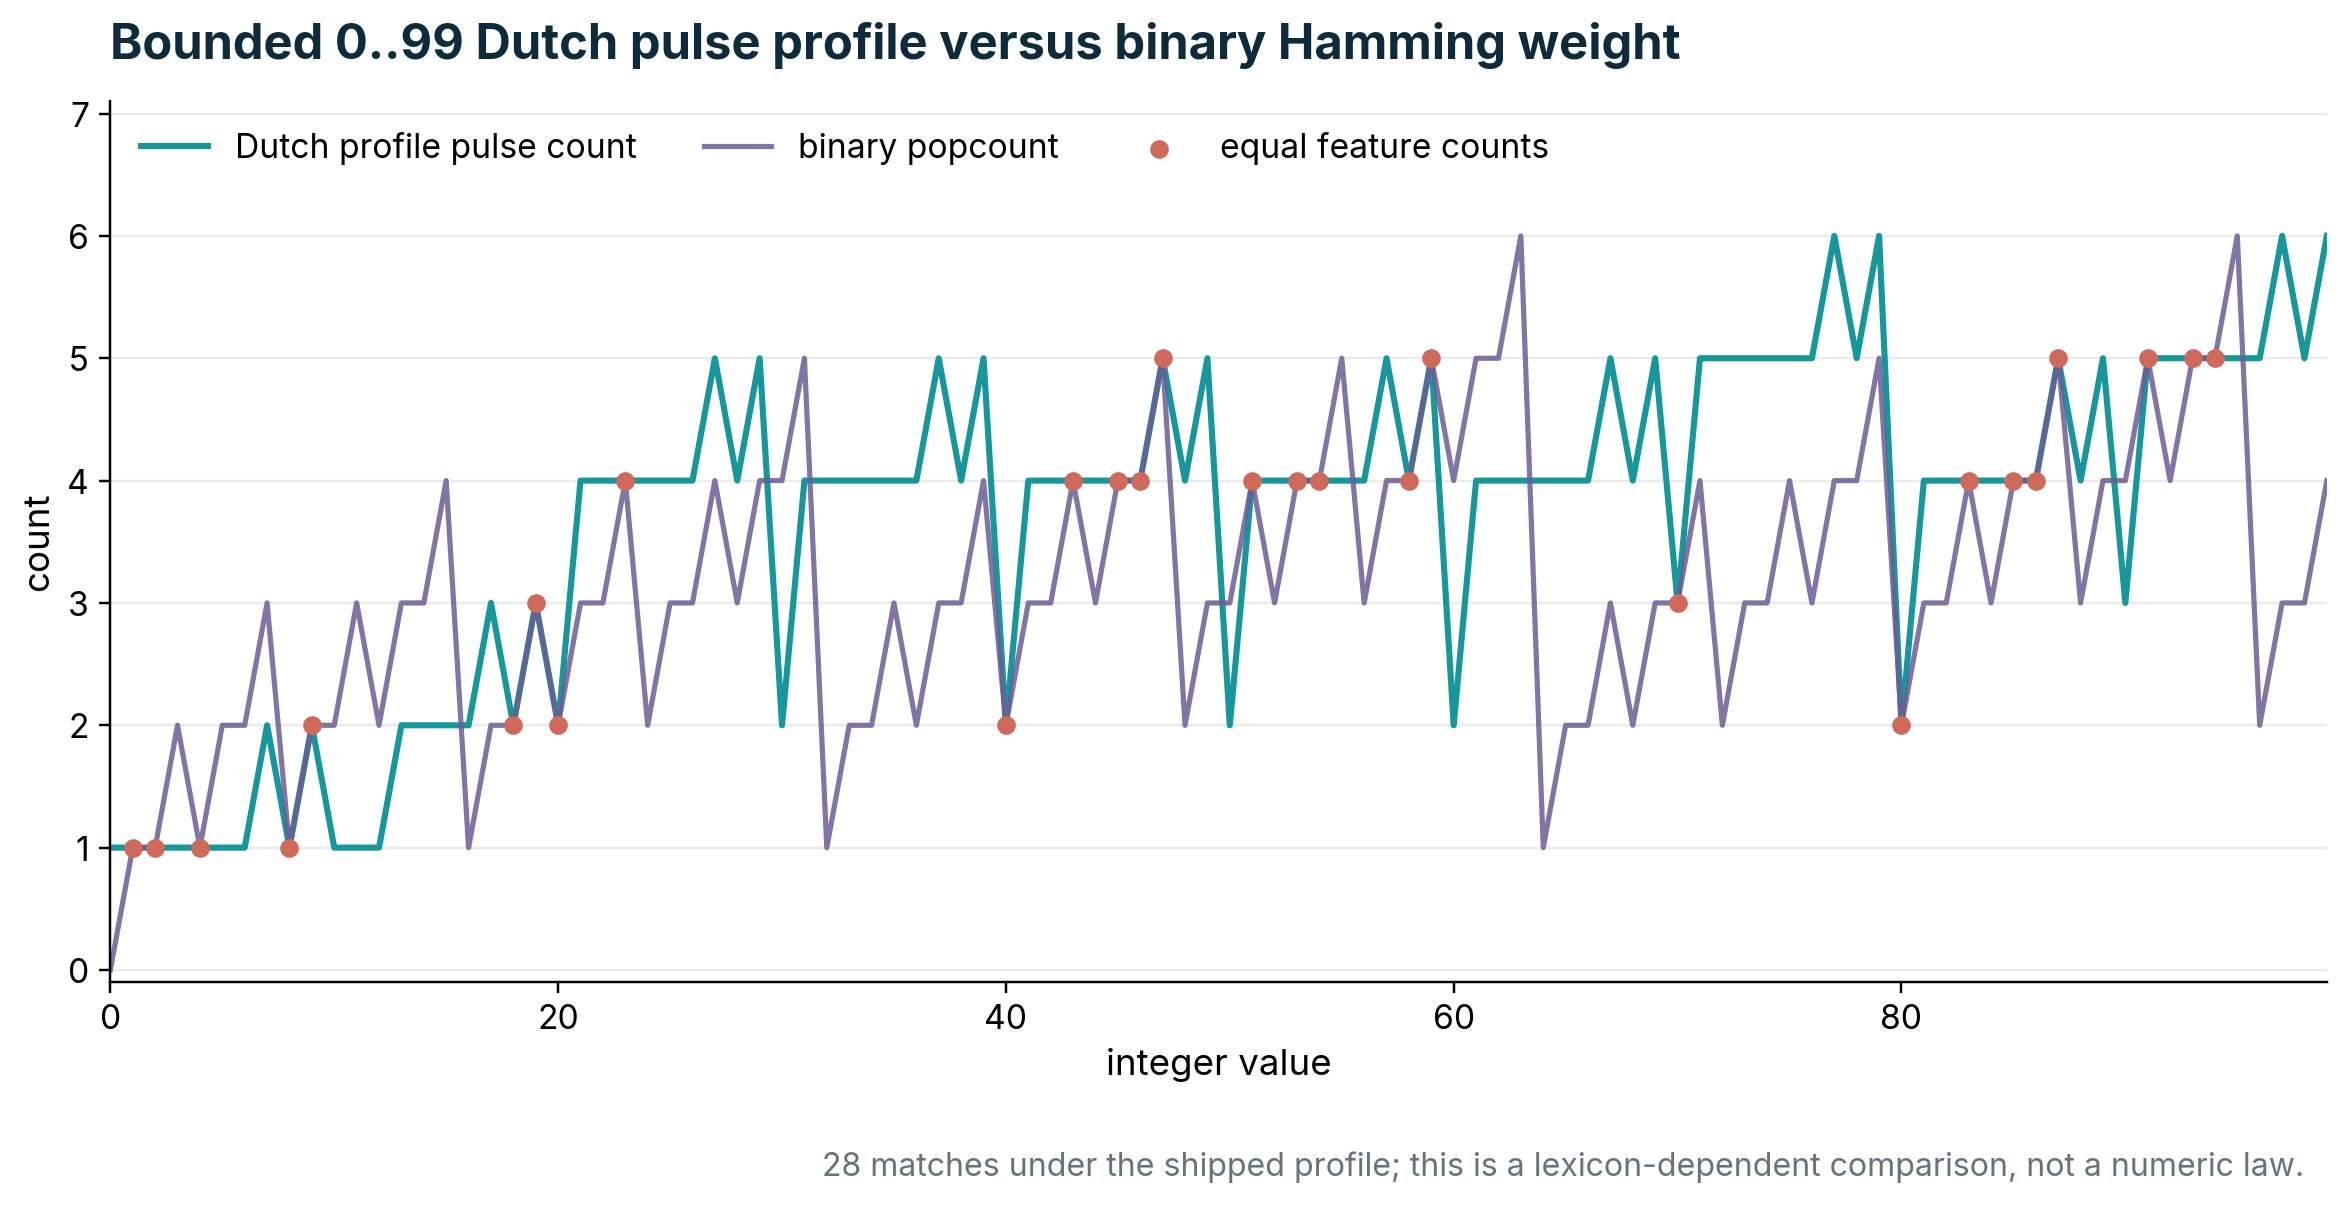
\includegraphics[width=0.96\textwidth]{dutch_number_atlas.png}
\caption{Profile pulse counts and binary Hamming weights across 0--99.}
\end{figure}

\subsection{Selected lexicon rows}
\begingroup
\small
\setlength{\tabcolsep}{3pt}
\begin{longtable}{r>{\raggedright\arraybackslash}p{3.0cm}>{\raggedright\arraybackslash}p{3.4cm}>{\raggedright\arraybackslash}p{2.7cm}>{\raggedright\arraybackslash}p{3.0cm}rr}
\toprule
\textbf{n} & \textbf{Orthography} & \textbf{Profile segments} & \textbf{Place order} & \textbf{Spoken order} & \textbf{syll.} & \textbf{pop} \\
\midrule
\endfirsthead
\toprule
\textbf{n} & \textbf{Orthography} & \textbf{Profile segments} & \textbf{Place order} & \textbf{Spoken order} & \textbf{syll.} & \textbf{pop} \\
\midrule
\endhead
0 & nul & nul & 0 & 0 & 1 & 0 \\
1 & een & een & 1 & 1 & 1 & 1 \\
2 & twee & twee & 2 & 2 & 1 & 1 \\
7 & zeven & ze | ven & 7 & 7 & 2 & 3 \\
9 & negen & ne | gen & 9 & 9 & 2 & 2 \\
10 & tien & tien & 10 & 10 & 1 & 2 \\
11 & elf & elf & 11 & 11 & 1 & 3 \\
12 & twaalf & twaalf & 12 & 12 & 1 & 2 \\
13 & dertien & der | tien & 10 | 3 & 3 | tien & 2 & 3 \\
17 & zeventien & ze | ven | tien & 10 | 7 & 7 | tien & 3 & 2 \\
18 & achttien & acht | tien & 10 | 8 & 8 | tien & 2 & 2 \\
19 & negentien & ne | gen | tien & 10 | 9 & 9 | tien & 3 & 3 \\
20 & twintig & twin | tig & 20 & 20 & 2 & 2 \\
21 & eenentwintig & een | en | twin | tig & 20 | 1 & 1 | en | 20 & 4 & 3 \\
23 & drieëntwintig & drie | en | twin | tig & 20 | 3 & 3 | en | 20 & 4 & 4 \\
27 & zevenentwintig & ze | ven | en | twin | tig & 20 | 7 & 7 | en | 20 & 5 & 4 \\
30 & dertig & der | tig & 30 & 30 & 2 & 4 \\
42 & tweeënveertig & twee | en | veer | tig & 40 | 2 & 2 | en | 40 & 4 & 3 \\
70 & zeventig & ze | ven | tig & 70 & 70 & 3 & 3 \\
99 & negenennegentig & ne | gen | en | ne | gen | tig & 90 | 9 & 9 | en | 90 & 6 & 4 \\
\bottomrule
\end{longtable}

\endgroup

\section{Kinematic calculus, guards and dynamics}

\subsection{Closed-form motion}
For constant acceleration,
\[
x(t)=p_0+v_0\Delta t+\tfrac12 a\Delta t^2,\qquad v(t)=v_0+a\Delta t.
\]
A geometric relation $f(x)=0$ becomes a temporal guard
\[
g(t)=f(x(t)).
\]
Selected line, plane, circle and sphere relations yield linear or quadratic roots for selected trajectories. Generic implicit-field/trajectory pairs require bracketed or certified numerical methods.

\subsection{Verified event condition}
The next valid event is
\[
t^*=\min\{t>t_0: R_j(q(t))=0,\;S_\alpha(q(t),t)=1,\;\chi(q(t),j,t)=1,\;conf\ge conf_{min}\}.
\]
The event record includes pre-state, post-state, relation residual, crossing direction, solver status, guard margin, confidence, route and lineage.

\subsection{Operation order}
The normative phases are:
\begin{enumerate}
\item parse literals and schemas;
\item normalize units, profiles and sign conventions;
\item resolve and verify definitions;
\item construct geometric and phonetic objects;
\item apply ordered transforms and hinges;
\item test local support;
\item test compatibility;
\item solve and certify relation guards;
\item commit transitions atomically;
\item append lineage and irreducible novelty.
\end{enumerate}

\begin{figure}[H]
\centering
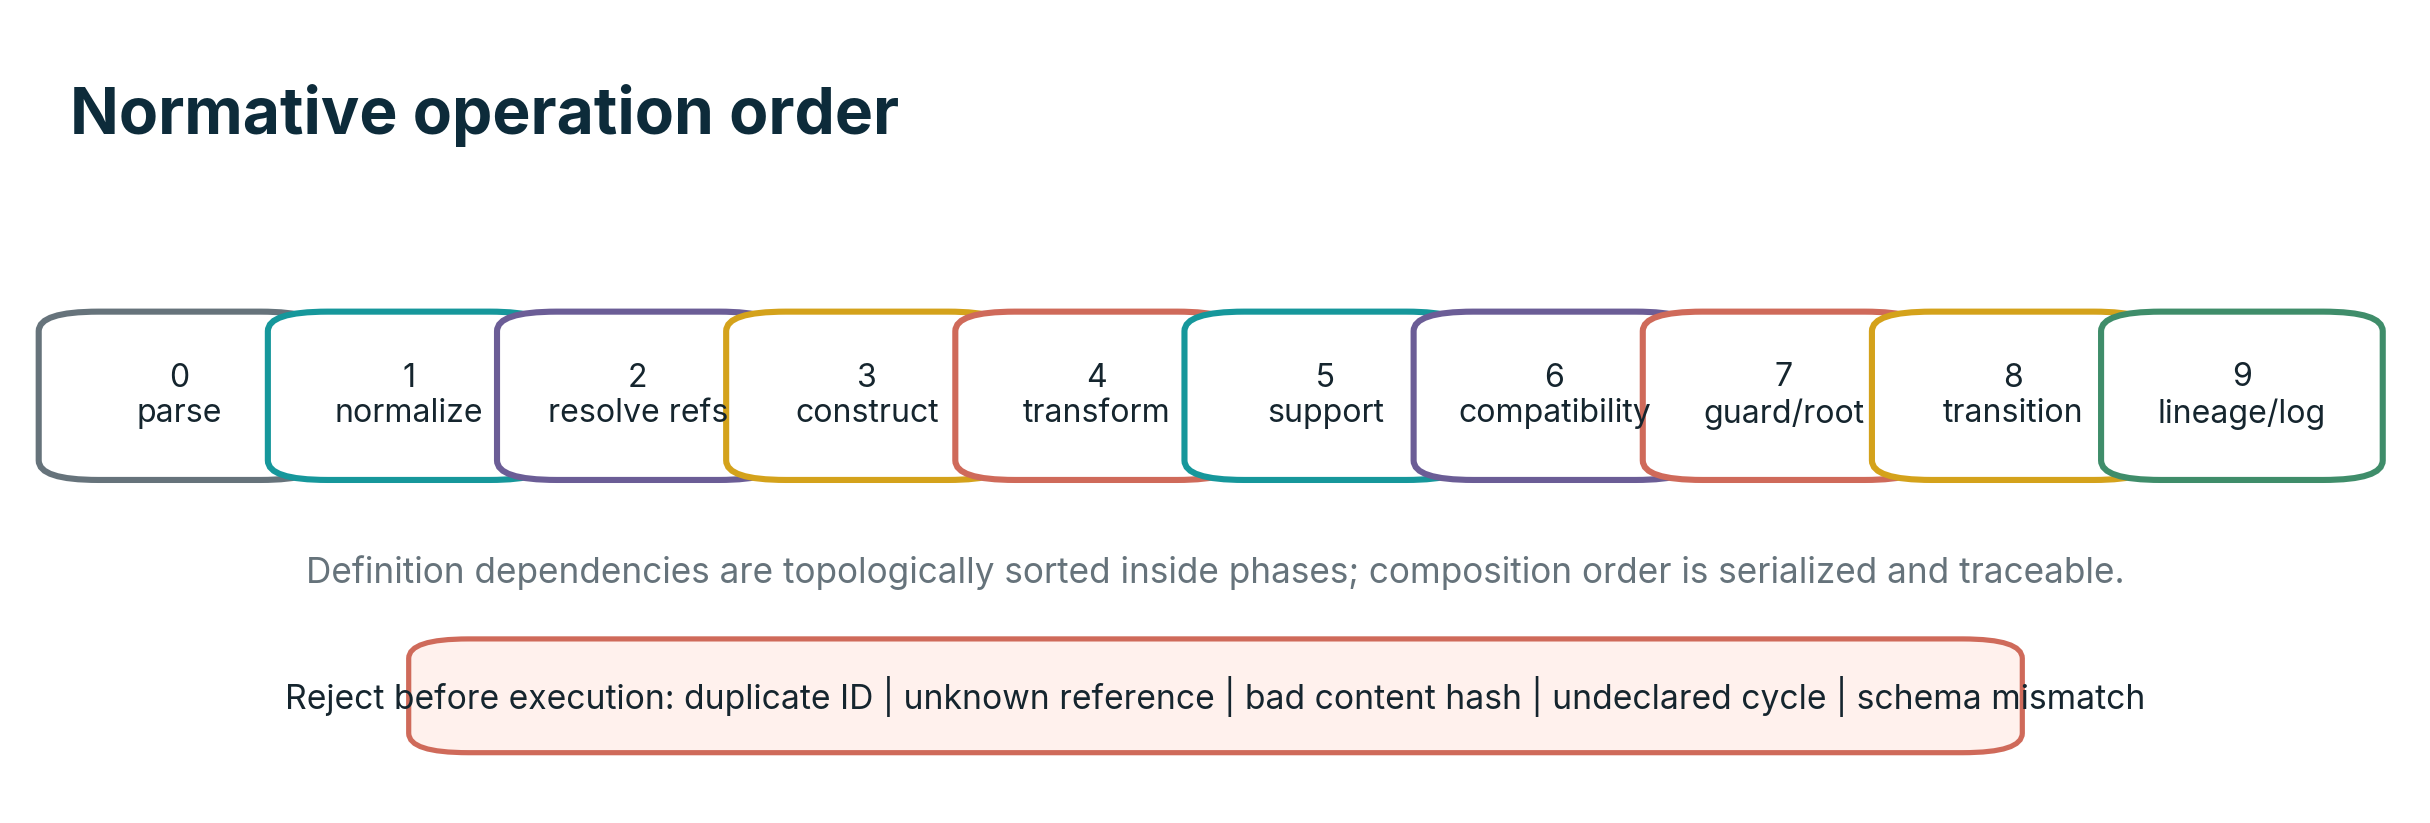
\includegraphics[width=0.98\textwidth]{evaluation_order.png}
\caption{The v3.6 evaluator makes mathematical order part of the substrate rather than hidden implementation detail.}
\end{figure}

\begin{boundarybox}
A field morph and a topology transition are not the same operation. Continuous interpolation may be evaluated in phase 4, while a topology-class change is committed only in phase 8 after support, compatibility and a verified guard.
\end{boundarybox}

\section{Reusable pattern library}
The 20 recipes below abstract the useful tricks away from the original dialogue subjects. Each recipe names a pipeline and a rule that can be reused for geometry, data structures, animation, procedural construction or event routing.

\begingroup
\small
\setlength{\tabcolsep}{2.5pt}
\begin{longtable}{>{\raggedright\arraybackslash}p{1.1cm}>{\raggedright\arraybackslash}p{3.5cm}>{\raggedright\arraybackslash}p{4.2cm}>{\raggedright\arraybackslash}p{7.2cm}}
\toprule
\textbf{ID} & \textbf{Pattern} & \textbf{Pipeline} & \textbf{Rule} \\
\midrule
\endfirsthead
\toprule
\textbf{ID} & \textbf{Pattern} & \textbf{Pipeline} & \textbf{Rule} \\
\midrule
\endhead
P36-01 & Radix threshold ladder & number -> thresholds & Use b\textasciicircum{}k boundaries as discrete scale events or shell indices. \\
\addlinespace[1.5pt]
P36-02 & Active-bit pulse simplex & integer -> set-bit pulses -> polygon & Embed sparse active positions as a chosen simplex or regular polygon while retaining bit positions as metadata. \\
\addlinespace[1.5pt]
P36-03 & Pascal parity mask & (n,k) -> C(n,k) mod 2 & Generate a Sierpinski occupancy mask with exact parity tests; do not claim generic power-of-two rows are all odd. \\
\addlinespace[1.5pt]
P36-04 & Dutch teen suffix hinge & 13..19 -> unit-root + tien & Represent morphological order separately from decimal place order. \\
\addlinespace[1.5pt]
P36-05 & Dutch en-order hinge & 21..99 non-multiple tens -> unit + en + tens & Insert a connector node and perform a two-component semantic transposition. \\
\addlinespace[1.5pt]
P36-06 & Cut-open boundary graph & closed edge -> cut port pair & Change a loop constraint into an open path with explicit endpoint identity. \\
\addlinespace[1.5pt]
P36-07 & Loop-to-leg morph & closed arc -> diagonal segment & Interpolate curve controls while separately recording the topology event. \\
\addlinespace[1.5pt]
P36-08 & Split-oval antisymmetry & single loop -> two branches & Use a fixed center node and opposite signed displacement fields. \\
\addlinespace[1.5pt]
P36-09 & Overlap-lens domain & A,B -> A intersection B & Treat overlap as geometry, tolerance, blend or join domain only after semantics are declared. \\
\addlinespace[1.5pt]
P36-10 & SDF-zero event & f(x(t)) -> root -> transition & Promote a boundary crossing from sampling detail to event semantics. \\
\addlinespace[1.5pt]
P36-11 & Cone support gate & position,axis,radius,angle -> admit/reject & Prune by radial and angular support before relation solving. \\
\addlinespace[1.5pt]
P36-12 & Nested-shell relevance & radius -> interval index & Use concentric intervals as local multiscale support, not global identity. \\
\addlinespace[1.5pt]
P36-13 & Mobius orientation wrap & boundary crossing -> coordinate wrap + orientation flip & Implement non-orientability as an explicit quotient map. \\
\addlinespace[1.5pt]
P36-14 & Klein sheet wrap & boundary crossing -> wrap + orientation and sheet update & Keep projected self-intersection distinct from state coupling. \\
\addlinespace[1.5pt]
P36-15 & Hourglass route table & guard locus + quadrant + parity -> branch & Route through a finite four-sector table. \\
\addlinespace[1.5pt]
P36-16 & Log-polar bitmask & Cartesian point -> core flag, rho, theta -> sector bit & Use a compact local admission mask with explicit dimensions and singular core. \\
\addlinespace[1.5pt]
P36-17 & Golden-angle schedule & index -> low-regularity angular sample & Use as a sample schedule only; no zero-aliasing or zero-cost claim. \\
\addlinespace[1.5pt]
P36-18 & Bounded grammar recursion & seed + productions + budgets -> definition graph & Stop on depth, symbol, expression or cycle limits. \\
\addlinespace[1.5pt]
P36-19 & Event-latched field morph & continuous alpha + discrete topology state & Keep visual interpolation and committed topology state separate. \\
\addlinespace[1.5pt]
P36-20 & Content-addressed definition graph & canonical records -> hashes -> dependency DAG & Make the substrate carry and verify its own operator definitions. \\
\addlinespace[1.5pt]
\bottomrule
\end{longtable}

\endgroup

\section{Literal example substrate}

\subsection{In-substrate definitions}
The example JSON includes definitions for a literal integer, binary radix encoding, active-bit filtering, a Dutch number lexeme, syllable pulses, count comparison, pulse polygon geometry, a Dutch connector hinge, a Möbius quotient, an SDF-zero event relation and the canonical evaluation schedule. Each record carries a content hash.

\begin{definitionbox}
The example is not pseudocode. It is accepted by the shipped JSON Schema, loaded by the reference runtime, topologically ordered, hash-verified and executed by the test suite.
\end{definitionbox}

\subsection{Schema excerpt}
\VerbatimInput[fontsize=\scriptsize,breaklines=true,breakanywhere=true,frame=single,rulecolor=\color{UGTSGrey},numbers=left,numbersep=4pt,firstline=1,lastline=58]{../examples/ugts_kc_3_6_example.json}

\subsection{Execution result}
For \code{number:19}, the trace ends with a three-vertex polygon and a feature comparison carrying the exact semantics \emph{feature-count coincidence; no numeric identity}. For \code{number:23}, it records spoken order \code{[3, "en", 20]} and a four-pulse polygon.

\section{Reference implementation and validation}

\subsection{Package modules}
\begin{center}
\begin{tabularx}{0.98\textwidth}{>{\ttfamily\scriptsize\raggedright\arraybackslash}p{4.6cm}X}
\toprule
src/ugts36/canonical.py & Canonical JSON, SHA-256 content addresses and hash verification. \\
src/ugts36/\allowbreak phonetics\_nl.py & Bounded Dutch 0--99 lexicon, hinges, pulse counts and feature matches. \\
src/ugts36/geometry.py & Radix operations, active bits, regular embeddings, affine hinges, log-polar chart, implicit fields and kinematics. \\
src/ugts36/topology.py & Dependency sorting, permutation hinges, Möbius/Klein maps, guard crossing and hourglass routing. \\
src/ugts36/model.py & Typed definition nodes, substrate loading, reference validation and dependency order. \\
src/ugts36/runtime.py & Minimal literal pipeline evaluator and deterministic trace. \\
tests/\allowbreak test\_ugts36.py & Thirty-six executable tests. \\
\bottomrule
\end{tabularx}
\end{center}

\subsection{Test result}
\VerbatimInput[fontsize=\scriptsize,breaklines=true,breakanywhere=true,frame=single,rulecolor=\color{UGTSGrey},firstline=1,lastline=46]{../test_results.txt}

The tests establish internal consistency of the bounded package. They verify canonical hashing, radix transitions, active bits, geometry embeddings, Dutch lexicon classes, the \emph{en} hinge, composition order, quotient maps, guard crossing, dependency cycles, JSON Schema validity and literal pipeline traces. They do not establish physical performance or universal linguistic laws.

\subsection{Reproduction commands}
\begin{Verbatim}[fontsize=\small,frame=single]
cd UGTS_KC_3_6_Tom_Klootwijk
PYTHONPATH=src python -m unittest discover -s tests -v
PYTHONPATH=src python examples/demo.py
\end{Verbatim}

\section{Claims ledger}
\begin{longtable}{>{\raggedright\arraybackslash}p{4.5cm}>{\raggedright\arraybackslash}p{2.4cm}>{\raggedright\arraybackslash}p{8.5cm}}
\toprule
\textbf{Claim or motif} & \textbf{Disposition} & \textbf{Technical treatment in 3.6} \\
\midrule
\endfirsthead
\toprule
\textbf{Claim or motif} & \textbf{Disposition} & \textbf{Technical treatment in 3.6} \\
\midrule
\endhead
Digit thresholds occur at radix powers. & SUPPORTED & Exact positional-number result; admitted as a shell/index event. \\
19 has binary Hamming weight three. & SUPPORTED & $19=16+2+1$ and \code{10011} has three set bits. \\
The shipped Dutch profile gives three pulses for \emph{negentien}. & BOUNDED & True under the explicit profile; dialect/tokenizer semantics are versioned. \\
Therefore 19 equals \code{111}. & REJECT & The active-bit projection has three ones; the numeric binary representation remains \code{10011}. \\
Three pulses can form a triangle. & ENGINEERING & A declared three-vertex embedding is valid; it is a chosen map. \\
Pascal parity produces a Sierpiński pattern. & SUPPORTED & Exact parity construction, with corrected row-index statement. \\
$\binom{5}{3}=10$ proves the decimal threshold. & DEMOTE & Correct combinatorial count, but no causal proof. \\
A log-polar LUT removes the origin singularity. & CORRECTED & Scaling becomes translation in $\rho$; an explicit core remains. \\
One-bit jitter eliminates aliasing. & REJECT & It may dither or shape error; quality and cost remain measurable. \\
A generic SDF gives exact distance everywhere. & CORRECTED & Only valid primitives/transforms claim exact-distance capability. \\
A one-bit hinge contains complete state. & REJECT & A bit selects route/map/validity; continuous state and lineage remain separate. \\
Topology creates energy or physical self-assembly. & REJECT & Topology is an explicit gluing/routing abstraction unless an independent physical model is supplied. \\
Personal dates or historical numbers are geometric invariants. & REJECT & They may be literal metadata, never promoted to causal geometry without an external model and evidence. \\
Definitions can refer to definitions. & SUPPORTED WITH BOUNDS & References must resolve, hashes verify and dependencies remain acyclic under v3.6. \\
Dutch \emph{en} acts as a structural hinge. & ENGINEERING & The connector is a typed graph node between unit and tens in the shipped spoken-order chart. \\
\bottomrule
\end{longtable}

\section{Acceptance and kill criteria}
UGTS-KC 3.6 should be rejected or simplified for a target system when any of the following occurs:
\begin{itemize}
\item definitions cannot be normalized to typed domains/codomains or stable content addresses;
\item unresolved references, ambiguous language profiles or cycles dominate the graph;
\item operation order changes results but is not recorded;
\item support and compatibility fail to prune enough candidate relations;
\item numerical error exceeds the event guard margin or changes event order;
\item morphology or phonetic segmentation is treated as universal rather than profile-bound;
\item a feature coincidence is used as a causal or physical conclusion;
\item event/branch density costs more than the materialization avoided;
\item a conventional data model is simpler, faster or more accurate at the same error budget.
\end{itemize}

\section{Conclusion}
The useful thread in the attached documents is not a hidden universal code. It is a family of practical transformations: radix thresholds, sparse active positions, parity patterns, boundary edits, local coordinate charts, implicit relations, guarded topology changes, explicit hinges and lineage-aware routing. Version 3.6 packages those transformations into the substrate itself. Every definition has a name, type, dependency set, phase, provenance and content hash; every instance references a definition; every pipeline records its order.

Dutch number language supplies a particularly clean structural example. The numeral \code{23} stores tens before units, while the spoken form \emph{drieëntwintig} places the unit before the tens word and joins them through \emph{en}. UGTS-KC 3.6 represents that difference as a chart map with a connector hinge. The same discipline keeps the 19/three-pulse observation useful without confusing a memorable pattern with arithmetic identity.

\begin{decisionbox}
Version 3.6 is ready as a bounded, inspectable and executable definition substrate. Its strongest upgrade is referential: the geometry, topology, hinge rules, language profile and operation order are no longer external explanations. They are literal, verifiable objects inside the substrate.
\end{decisionbox}

\clearpage
\appendix
\section{Complete v3.6 operator catalog}
The 36 mechanisms below are the version 3.6 delta namespace. They do not silently renumber the 197-mechanism baseline documented by the supplied GPU-native addendum.

\begingroup
\scriptsize
\setlength{\tabcolsep}{2.5pt}
\renewcommand{\arraystretch}{1.08}
\begin{longtable}{>{\raggedright\arraybackslash}p{1.0cm}>{\raggedright\arraybackslash}p{2.4cm}>{\raggedright\arraybackslash}p{3.2cm}>{\raggedright\arraybackslash}p{7.1cm}>{\raggedright\arraybackslash}p{2.3cm}}
\toprule
\textbf{ID} & \textbf{Domain} & \textbf{Mechanism} & \textbf{Normalized technical definition} & \textbf{Disposition / validation} \\
\midrule
\endfirsthead
\toprule
\textbf{ID} & \textbf{Domain} & \textbf{Mechanism} & \textbf{Normalized technical definition} & \textbf{Disposition / validation} \\
\midrule
\endhead
K36-01 & Referential core & Literal definition node & A geometry, topology, operator, profile or schedule is stored as a typed definition record inside the substrate. & RETAIN / Schema + tests \\
\addlinespace[1.5pt]
K36-02 & Referential core & Content-addressed definition & Canonical UTF-8 JSON, excluding the hash field itself, is hashed with SHA-256 to make definition identity verifiable. & ENGINEERING / Implemented \\
\addlinespace[1.5pt]
K36-03 & Referential core & Explicit dependency edge & Every composed definition lists definition IDs it depends on; hidden imports and implicit global state are forbidden. & RETAIN / Implemented \\
\addlinespace[1.5pt]
K36-04 & Referential core & Versioned namespace & Definition IDs include stable namespaces while schema\_version and profile\_version separate compatible from incompatible semantics. & RETAIN / Schema \\
\addlinespace[1.5pt]
K36-05 & Referential core & Definition-instance separation & A definition describes an operator or shape family; an instance supplies literal parameters and state through definition\_ref. & RETAIN / Schema + runtime \\
\addlinespace[1.5pt]
K36-06 & Referential core & Acyclic resolution rule & Definition dependency graphs must be acyclic unless a future fixed-point kind declares bounds, tolerance and termination. & BOUNDED / Cycle rejection tested \\
\addlinespace[1.5pt]
K36-07 & Geometry & Typed implicit-field sign & An implicit field declares domain, codomain and sign convention: negative interior, zero boundary, positive exterior. & RETAIN / Specified \\
\addlinespace[1.5pt]
K36-08 & Geometry & Exact-SDF capability flag & Exact signed-distance status is a capability that only valid primitives and distance-preserving transforms may claim. & CORRECTED / Schema guard \\
\addlinespace[1.5pt]
K36-09 & Geometry & Parametric curve and sweep & A curve gamma(u) and a frame or transport rule may generate a swept surface; parameter interval and regularity are explicit. & ENGINEERING / Specified \\
\addlinespace[1.5pt]
K36-10 & Geometry & Pulse polygon embedding & m declared pulses map to a point, segment or regular m-gon; for m=3 the result is a triangle. & ENGINEERING / Implemented \\
\addlinespace[1.5pt]
K36-11 & Geometry & Radix shell chart & Digit thresholds b\textasciicircum{}k form exact scale boundaries and may index nested shells without implying that space is inherently radix-based. & RETAIN / Implemented \\
\addlinespace[1.5pt]
K36-12 & Geometry & Log-polar core chart & rho=ln(r/r0), theta=atan2(y,x) is local and carries an explicit core/singularity flag. & RETAIN / Implemented \\
\addlinespace[1.5pt]
K36-13 & Topology & Explicit quotient/gluing map & Topology is represented by boundary ports, coordinate maps, orientation transport and optional sheet changes. & RETAIN / Implemented examples \\
\addlinespace[1.5pt]
K36-14 & Topology & Sheet-aware co-location & Equal coordinates do not imply equality or coupling; sheet, phase, orientation, branch and policy remain typed state. & RETAIN / Schema \\
\addlinespace[1.5pt]
K36-15 & Topology & Orientation transport & Orientation is propagated independently and flips only at declared maps or transitions. & RETAIN / Mobius/Klein tests \\
\addlinespace[1.5pt]
K36-16 & Topology & Port and branch routing & A guarded crossing selects an explicit output port and branch; the routing table is finite and inspectable. & RETAIN / Specified \\
\addlinespace[1.5pt]
K36-17 & Topology & Split-merge lineage & Splits create child addresses and merges record all parents; coordinates never replace durable identity. & RETAIN / Schema \\
\addlinespace[1.5pt]
K36-18 & Topology & Guarded topology change & A morph may vary continuously, but a topology-class change commits only at an event with a declared guard and transition. & CORRECTED / Specified \\
\addlinespace[1.5pt]
K36-19 & Hinge calculus & Generic hinge tuple & A hinge is H=(pivot,state,map,guard,invariant) with typed continuous or discrete state. & ENGINEERING / Specified \\
\addlinespace[1.5pt]
K36-20 & Hinge calculus & Continuous planar hinge & A continuous hinge uses an affine rotation about a fixed pivot; velocity follows the derivative of the transform. & RETAIN / Implemented \\
\addlinespace[1.5pt]
K36-21 & Hinge calculus & Discrete parity hinge & A one-bit state selects one of two declared maps or routes and does not carry full geometry or identity. & RETAIN / Implemented \\
\addlinespace[1.5pt]
K36-22 & Hinge calculus & Connector hinge & A zero-magnitude connector can be topologically necessary in an ordered parse graph, as with Dutch en. & ENGINEERING / Lexicon-tested \\
\addlinespace[1.5pt]
K36-23 & Hinge calculus & Non-commutative hinge chain & Composition order is explicit because H2$\circ$H1 generally differs from H1$\circ$H2. & RETAIN / Tested \\
\addlinespace[1.5pt]
K36-24 & Hinge calculus & Invariant subspace contract & A hinge may declare fixed points, axes or quantities; the runtime validates them instead of inferring invariance from a name. & ENGINEERING / Specified \\
\addlinespace[1.5pt]
K36-25 & Dutch phonetics & Bounded Dutch number profile & A versioned lexicon covers standard 0..99 orthography, pronunciation-like segments, morphemes and hinge metadata. & BOUNDED / 100 entries generated \\
\addlinespace[1.5pt]
K36-26 & Dutch phonetics & Syllable-pulse operator & Each declared pronunciation segment emits one pulse; dialect and tokenizer are profile metadata. & ENGINEERING / Implemented \\
\addlinespace[1.5pt]
K36-27 & Dutch phonetics & Teen suffix hinge & For regular 13..19 forms, the unit root precedes tien although decimal place semantics are ten plus unit. & RETAIN / Lexicon-tested \\
\addlinespace[1.5pt]
K36-28 & Dutch phonetics & En connector hinge & For non-multiple tens 21..99, spoken morphology is unit-en-tens while numeral place order is tens-unit. & RETAIN / Lexicon-tested \\
\addlinespace[1.5pt]
K36-29 & Dutch phonetics & Spoken-place permutation & The place tuple and spoken tuple are separate charts connected by an explicit permutation plus optional connector node. & ENGINEERING / Implemented \\
\addlinespace[1.5pt]
K36-30 & Dutch phonetics & Feature-count comparison & Binary popcount and phonetic pulse count may be compared; equality is tagged as a coincidence, never numeric identity. & CORRECTED / Implemented \\
\addlinespace[1.5pt]
K36-31 & Evaluation & Phase-ordered evaluator & The canonical order is parse, normalize, resolve, construct, transform, support, compatibility, guard, transition, lineage. & ENGINEERING / Schedule shipped \\
\addlinespace[1.5pt]
K36-32 & Evaluation & Support-compatibility-guard discipline & Cheap local support precedes compatibility; event solving occurs only after both gates admit a candidate. & RETAIN / Runtime rule \\
\addlinespace[1.5pt]
K36-33 & Evaluation & Deterministic trace & Each pipeline step records definition ID, operator kind and typed output to make order and provenance inspectable. & RETAIN / Runtime + demo \\
\addlinespace[1.5pt]
K36-34 & Evaluation & Evidence disposition & Every source-derived or newly inferred mechanism is labeled RETAIN, ENGINEERING, CORRECTED, BOUNDED, DEMOTE or REJECT. & RETAIN / Catalog \\
\addlinespace[1.5pt]
K36-35 & Evaluation & Unknown-reference and cycle rejection & Loading fails on missing definition IDs, duplicate IDs, invalid hashes or cyclic dependencies. & RETAIN / Tests \\
\addlinespace[1.5pt]
K36-36 & Evaluation & Package verification contract & Schema validation, executable tests, source hashes, file hashes and a reproducible demo accompany the PDF. & RETAIN / Delivered \\
\addlinespace[1.5pt]
\bottomrule
\end{longtable}

\endgroup

\section{Source register and hashes}
\begin{longtable}{>{\raggedright\arraybackslash}p{1.3cm}>{\raggedright\arraybackslash}p{5.5cm}>{\raggedright\arraybackslash}p{9.0cm}}
\toprule
\textbf{ID} & \textbf{Source} & \textbf{SHA-256 and role} \\
\midrule
SRC-A & Dutch-number dialogue Markdown & \texttt{\seqsplit{7aa55d4f03e07c6ec058b1dd05554c03730d0f6263803b9364fe34ccce6c1851}}. Source for phonetic, radix, active-bit, triangle, fractal, log-polar, hinge and claims-boundary analysis. \\
SRC-B & Unified Geometric-Topological Substrate (UGTS-0) & \texttt{\seqsplit{c991aba24cc939ba680697b62b9e19545131cf34060793490bf149c6e2ab522e}}. Primary query-first architecture, relation/event calculus, topology and evidence boundary. \\
SRC-C & UGTS-GN 1.1 GPU-native addendum & \texttt{\seqsplit{3a6b6c57118ca4e2d7d7e577508c3477a095d133791f3708cb56a054285225d2}}. Normalized catalog, narrow one-bit semantics, precision, ABI, validation and claims ledger. \\
\bottomrule
\end{longtable}

The raw uploaded sources are not duplicated in the package. The ZIP contains hashes and normalized source notes so that technical traceability is preserved without reproducing unrelated personal or narrative material.

\section{Package layout}
\begin{Verbatim}[fontsize=\scriptsize,frame=single]
UGTS_KC_3_6_Tom_Klootwijk/
  README.md
  CHANGELOG.md
  NOTICE.md
  VERSION
  pyproject.toml
  validation_report.json
  report/UGTS_KC_3_6.pdf
  report/UGTS_KC_3_6.tex
  report/figures/*.png
  spec/ugts_kc_3_6.schema.json
  spec/operator_catalog_3_6.{csv,json}
  spec/pattern_recipes_3_6.{csv,json}
  data/dutch_numbers_0_99.{csv,json}
  data/dutch_binary_pulse_matches_0_99.csv
  examples/ugts_kc_3_6_example.json
  examples/demo.py
  examples/demo_output.json
  src/ugts36/*.py
  tests/test_ugts36.py
  test_results.txt
  sources/source_register.json
  sources/source_analysis.md
  checksums/SHA256SUMS.txt
\end{Verbatim}

\end{document}
